\documentclass[aspectratio=169,xcolor=dvipsnames]{beamer}
\usetheme{SimplePlus}

% Math
\usepackage{nicefrac}

% Tipography stuff
\usepackage{booktabs} % Allows the use of \toprule, \midrule and \bottomrule in tables
\usepackage[english]{babel}
\usepackage{csquotes}
\usepackage{microtype}
\usepackage{pdfpages}
\usepackage{fontawesome5}
\usepackage{soul}
\usepackage{euler}
\usepackage{algorithm2e}
\usepackage{animate}
\usepackage{ifthen}
\usepackage{multirow}
\usepackage{multicol}
\usepackage{pgfplotstable}

% Bibliography
\usepackage[giveninits,style=authoryear-comp,backend=biber]{biblatex}
\addbibresource{../fracbiblio.bib}
\newcommand\unnumbered{\setbeamertemplate{footline}{}}%\addtocounter{framenumber}{-1}
\renewcommand*{\bibfont}{\normalfont\small}

% Figures
\usepackage{tikz,pgfplots}
\usetikzlibrary{calc,arrows,patterns,matrix,external}
\usepackage{subfig}
\usepackage{graphicx} % Allows including images
\usepackage[american]{circuitikz}
\usepackage{tikz-network}
\tikzexternalize[prefix=Figures/] % activate and define figures/ as cache folder
\usepackage{mathtools}

% Links
\usepackage{hyperref}
\hypersetup{colorlinks,linkcolor=,urlcolor=MidnightBlue}

% Code
\usepackage{minted}

% Block matrices
\newcommand{\bigzero}{\mbox{\normalfont\Large\bfseries 0}}
\newcommand{\rvline}{\hspace*{-\arraycolsep}\vline\hspace*{-\arraycolsep}}
\newcommand{\R}{\mathbb{R}}
\newcommand{\bone}{{\bf 1}}
\newcommand{\evec}{{\bf e}}
\newcommand{\dvec}{{\bf d}}
\newcommand{\xvec}{{\bf x}}
\newcommand{\yvec}{{\bf y}}
\newcommand{\qvec}{{\bf q}}
\newcommand{\svec}{{\bf s}}
\newcommand{\pvec}{{\bf p}}
\newcommand{\tvec}{{\bf t}}
\definecolor{Ao}{rgb}{0.0, 0.5, 0.0}
\setlength{\tabcolsep}{0.3em}


\author{Fabio Durastante}
\title{An introduction to fractional calculus}
\subtitle{Fundamental ideas and numerics}
\institute{Università di Pisa\\\href{mailto:fabio.durastante@unipi.it}{\faEnvelope\;fabio.durastante@unipi.it}\\\href{https://fdurastante.github.io}{\faFirefox\;fdurastante.github.io}}
\date{October, 2022}

\newcommand{\de}{{\rm d}}


\begin{document}
	
	{\unnumbered
		\begin{frame}[t,plain,noframenumbering]
			\titlepage
			\vspace{-4em}
\includegraphics[width=2cm]{frame.png}
		\end{frame}
	}

	\section{All-at-once}

	\begin{frame}{All-at-once}
	We have seen that for a problem of the form
	\[
	\begin{cases}
		\only<1>{u_t = \mathcal{L}(u), & u \,:\; \Omega \times [0,T] \rightarrow \mathbb{R}^d, \; \Omega \subseteq \mathbb{R}^d \\}
		\only<2>{\mathbf{u}_t = \mathcal{L}_h(\mathbf{u}), & \mathbf{u}\,:\;\mathbb{R}^n \times [0,T] \rightarrow \mathbb{R}^{n} \\}
		\only<1>{u(\mathbf{x},0) = u_0(\mathbf{x}),\\}
		\only<2>{\mathbf{u}(0)=\mathbf{u}_0,\\}
		\only<1>{\mathcal{B}(u) = 0, & \mathbf{x} \in \partial \Omega.}
		\only<2>{\mathcal{B}_h(\mathbf{u})=0.}
	\end{cases}
	\]
	with
	\begin{itemize}
		\item[\faCog] $\mathcal{L}(\cdot)$ a \emph{linear} and \emph{autonomous} differential operator (possibly involving fractional derivatives),
		\item[\faHammer] or changing $u_t$ with ${}^{CA}D_{[0,t]}^\alpha u$,
	\end{itemize}
	we can \alert{\textbf{rewrite it}} as a single linear system/matrix equation.\vfill
	
	\onslide<2>{To \emph{abstract the procedure} let's think about working the \alert{\textbf{M}}ethod \alert{\textbf{O}}f \alert{\textbf{L}}ine way!}
	\end{frame}

	\begin{frame}{All-at-once: system of autonomous ODE}
	Following the MOL trail, we now have to solve a \alert{system of autonomous ODEs}:
	\[
	M \mathbf{u}_t(t) = L \mathbf{u}(t), \qquad M,L \in \mathbb{R}^{n \times n}, 
	\]
	\begin{itemize}
		\item[\faHammer] that could be a \textbf{d}ifferential-\textbf{a}lgebraic system of \textbf{e}quations (DAE) if $\det(M) = 0$.
		\item[\faCog]<2-> To formulate the \emph{all-at-once} procedure, one has to select a method to \emph{march in time} the solution:
		\begin{itemize}
			\item[\faWrench]<3-> \normalsize Linear multistep methods,
			\item[\faWrench]<3-> \normalsize Runge-Kutta methods,
			\item[\faWrench]<3-> \normalsize General linear methods (a mix of the two above strategies).
		\end{itemize}
	\end{itemize}
	\end{frame}

	\subsection{Linear Multistep Methods (LMM)}
	
	\begin{frame}{Linear Multistep Methods}
	Given a general ODE of the form
	\[
		u'(t)=f(t,u(t)), \quad u(t_0)=u_0,
	\]
	a $k$-step LMM is a recursion of the form with step-size $h = t_{n+k} - t_{n+k-1} > 0$
	\[
	\sum_{j=0}^k \alpha_j u_{n+j}=\sum_{j=0}^k h \beta_j f_{n+j}, \qquad f_m  \triangleq f(t_m, y_m),
	\]
	with coefficients $\alpha_j\in\mathbb{R}$ and $\beta_j\in \mathbb{R}$ ($j=0, \ldots, k$), and we are \textbf{interested only} in \textbf{implicit methods}, i.e., $\beta_k\ne 0$.\vfill
	
	\onslide<2>{
	They can be analyzed by looking at the \textbf{polynomials}
	\[
	\rho(\zeta) = \sum_{j=0}^k \alpha_{j}\zeta^j = (\zeta - 1) \sum_{j=0}^{k-1} \gamma_{j}\zeta^j = (\zeta-1)\cdot \rho_R(\zeta),\qquad \sigma(\zeta) = \sum_{j=0}^k \beta_{j}\zeta^j.
	\]
	}
	
	\end{frame}

	\begin{frame}{Linear Multistep Methods}
	
	\begin{block}{$0$-stable method}
	A method is $0$-stable if all roots of $\rho(\zeta)= (\zeta-1)\cdot \rho_R(\zeta) = 0$ lie inside or on the unit circle, with no multiple unimodular roots.
	\end{block}
	
	\begin{itemize}
		\item[\faHammer] \textit{Zero stability} is necessary for convergence,
		\item[\faWrench] It is a condition on the \textit{extraneous operator} $\rho_R(\zeta)$, i.e., a condition on the $k$ coefficients $\{\gamma_j\}_{j=0}^{k-1}$.
	\end{itemize}

	\begin{block}<2->{$A$-stable method}
	The behavior of these methods can be analyzed by applying them on the \alert{test problem} $y' = k y$ subject to the initial condition $y(0)=1$ with $k\in \mathbb{C}$. The solution of this equation is $y(t)=e^{kt}$. If the numerical method exhibits the same behavior of the solution for a fixed step size, then the method is said to be $A$-stable.
	\end{block}

	\begin{itemize}
		\item[\faSadTear]<3-> Usually one ends up with limitations involving the admissible $h$.
	\end{itemize}
	
	\end{frame}

	\begin{frame}{Linear Multistep Methods: initial values}
	
	If we use a LMM with $k > 1$ we need \alert{more starting values} than the one we have!\vfill
	
	We are interested in \textbf{diffusion dominated problems}, thus \textbf{B}ackward-\textbf{D}ifferentiation \textbf{F}ormula\textbf{s} are a common choice.\vfill
	
	\begin{columns}
	\begin{column}{0.7\columnwidth}
	\begin{tabular}{c*{7}r}
		\toprule
		& \multicolumn{7}{c}{$\{\alpha_k\}_k$, $\beta_k = 1$, $\beta_j = 0$, $j \leq k$} \\
		\midrule
		\alert<1>{\textbf{BDF2}} & & & & & $1/2$ & $-2$ & ${3/2}$ \\
		\alert<2>{\textbf{BDF3}} & & & & $-1/3$ & $3/2$ & $-3$ & ${11/6}$ \\
		\alert<3>{\textbf{BDF4}} & & & $1/4$ & $-4/3$ & $3$ & $-4$ & ${25/12}$ \\
		\alert<4>{\textbf{BDF5}} & & $-1/5$ & $5/4$ & $-10/3$ & $5$ & $-5$ & ${137/60}$ \\
		\alert<5>{\textbf{BDF6}} & $1/6$ & $-6/5$ & $15/4$ & $-20/3$ & $15/2$ & $-6$ & ${147/60}$ \\
		\bottomrule
	\end{tabular}
	\end{column}
	\begin{column}{0.3\columnwidth}
	\only<1>{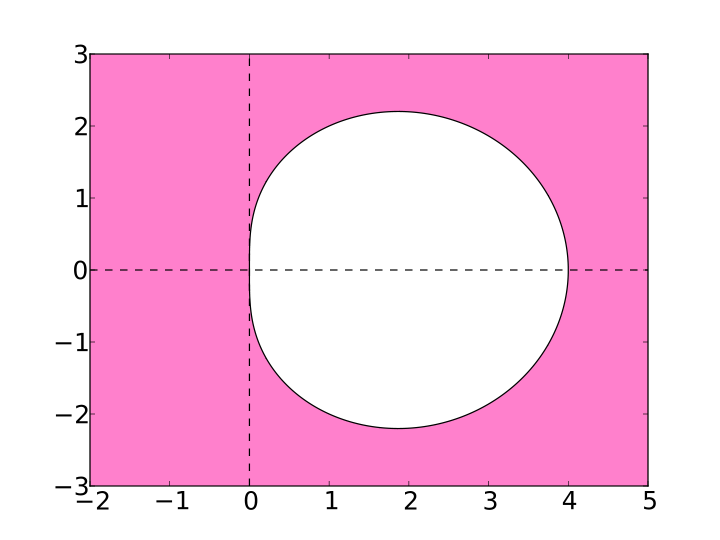
\includegraphics[width=\columnwidth]{720px-Stability_region_for_BDF2.svg.png}}%
	\only<2>{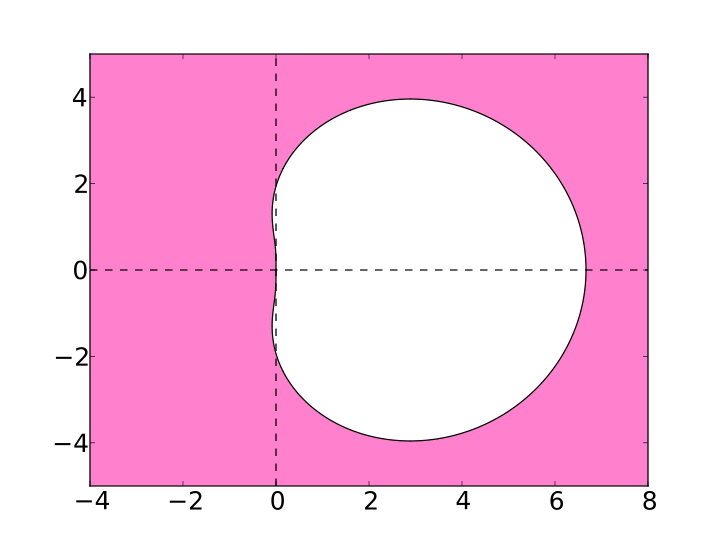
\includegraphics[width=\columnwidth]{720px-Stability_region_for_BDF3.svg.png}}%
	\only<3>{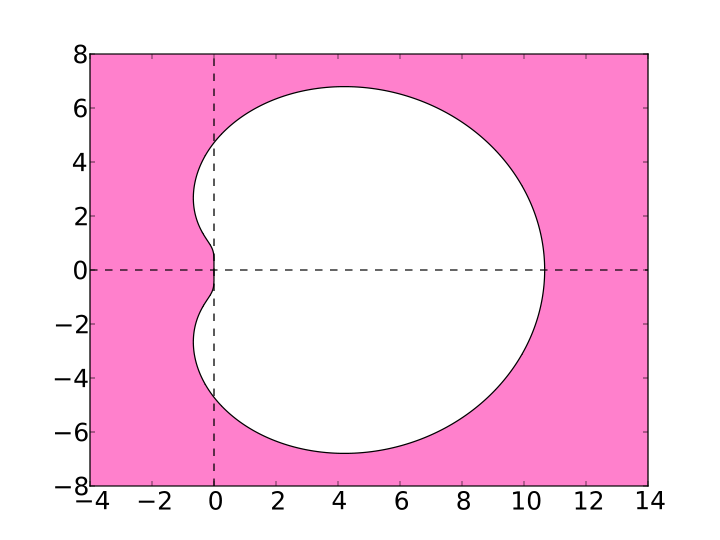
\includegraphics[width=\columnwidth]{720px-Stability_region_for_BDF4.svg.png}}%
	\only<4>{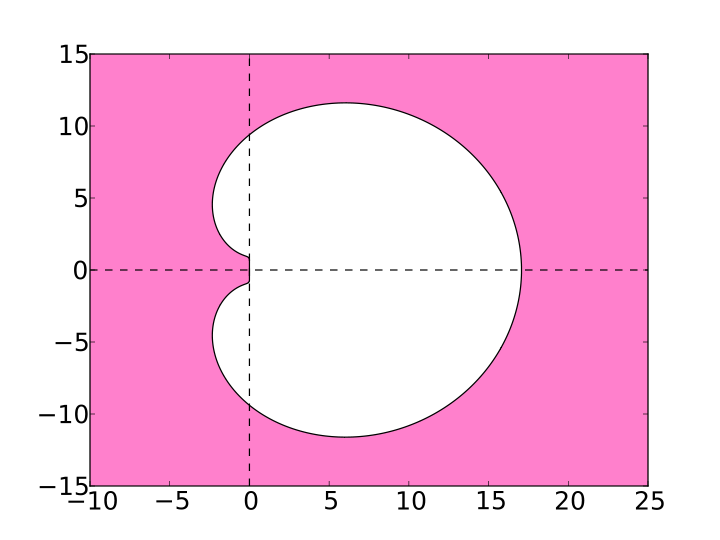
\includegraphics[width=\columnwidth]{720px-Stability_region_for_BDF5.svg.png}}%
	\only<5>{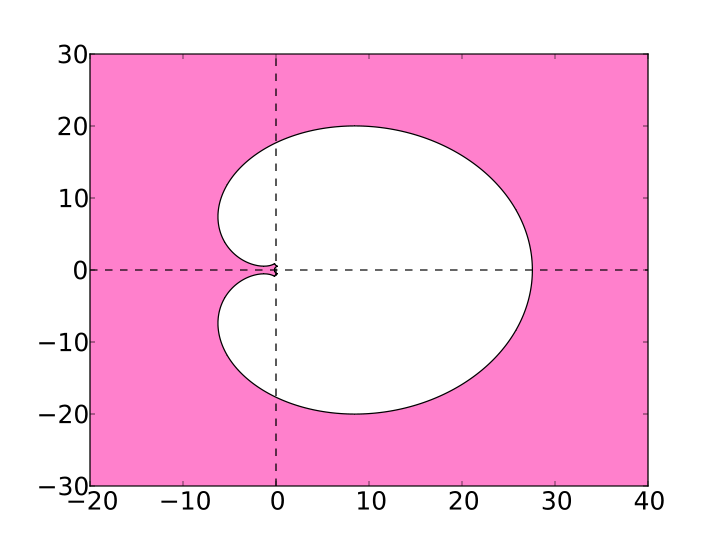
\includegraphics[width=\columnwidth]{720px-Stability_region_for_BDF6.svg.png}}%
	\end{column}
	\end{columns}\vfill

	\begin{itemize}
	\item[\faHammer] Methods with $k > 6$ are not zero-stable so they cannot be used.
	\item[\faWrench]<2-> If we want to use BDF6 we need 5 initial conditions, and have only one.
	\item[\faHammer]<2-> We can use lower order BDFs to generate the step we need.
\end{itemize}	
	\end{frame}

	\begin{frame}{Linear Multistep Methods}
	From what we have seen in the last lectures we can write down the problem as
	\[
	(\alert<2>{A_m} \otimes M_n - h \alert<3>{B_m} \otimes L_n) \mathbf{u} = \alert<4>{\mathbf{f}},
	\]
	\begin{onlyenv}<2>
	\[
	A_m = \begin{bmatrix}
	1 & \\
	-2 & \nicefrac{3}{2} \\
	\nicefrac{3}{2} & -3 & \nicefrac{11}{6} \\
	 -\nicefrac{4}{3} & 3 & -4 & \nicefrac{25}{12} \\
	 \nicefrac{5}{4} & -\nicefrac{10}{3} & 5 & -5 & \nicefrac{137}{60} \\
	-\nicefrac{6}{5} & \nicefrac{15}{4} & -\nicefrac{20}{3} & \nicefrac{15}{2} & -6 & \nicefrac{147}{60} \\
	\nicefrac{1}{6} & -\nicefrac{6}{5} & \nicefrac{15}{4} & -\nicefrac{20}{3} & \nicefrac{15}{2} & -6 & \nicefrac{147}{60} \\
	\vdots & \ddots & \ddots & \ddots & \ddots & \ddots & \ddots & \ddots \\
	\end{bmatrix}_{(m-1) \times (m-1)}
	\]
	\end{onlyenv}
	\begin{onlyenv}<3>
	\[
	B_m = \begin{bmatrix}
	1 & \\
	& 1 \\
	& & \ddots \\
	& & & 1
	\end{bmatrix}_{(m-1) \times (m-1)}
	\]
	\end{onlyenv}
	\begin{onlyenv}<4>
	\[
	\textbf{f} = \begin{bmatrix}
	\mathbf{u}_0 + f(t_{1})\\
	-\nicefrac{1}{2} \mathbf{u}_0 + f(t_{2})\\
	\nicefrac{1}{3} \mathbf{u}_0 + f(t_{3})\\
	-\nicefrac{1}{4} \mathbf{u}_0 + f(t_{4})\\
	\nicefrac{1}{5} \mathbf{u}_0 + f(t_{5})\\
	-\nicefrac{1}{6} \mathbf{u}_0 + f(t_{6})\\
	f(t_{7}) \\
	\vdots
	\end{bmatrix}
	\]
	\end{onlyenv}
	\end{frame}

\begin{frame}[fragile]{A simple example}
\begin{columns}
\begin{column}{0.59\columnwidth}\definecolor{bg}{rgb}{0.95,0.95,0.95}
\begin{minted}[bgcolor=bg,fontsize=\small,breaklines]{matlab}
L = [-2, 1; 0, -3]; % Problem
y0 = [1;1];
n = length(L);
% Discretize
m = 100;
T = linspace(0,10,m); h = T(2)-T(1);
r = zeros(m-1,1); c = zeros(m-1,1);
r(1:7)=[147/60,-6,15/2,-20/3,15/4,-6/5,1/6];
c(1) = 147/60;
A = toeplitz(r,c);
A(1,1) = 1; % Fix BCs
A(2,1) = -2; A(2,2) = 3/2;
A(3,1) = 3/2; A(3,2) = -3; A(3,3) = 11/6;
A(4,1) = -4/3; A(4,2) = 3; A(4,3) = -4; A(4,4) = 25/12;
A(5,1) = 5/4; A(5,2) = -10/3; A(5,3) = 5; 
\end{minted}
\end{column}
\begin{column}{0.39\columnwidth}\definecolor{bg}{rgb}{0.95,0.95,0.95}
\begin{minted}[bgcolor=bg,fontsize=\small,breaklines]{matlab}
A(5,4) = -5; A(5,5) = 137/60;
In = speye(n,n);
Im = speye(m-1,m-1);
%% Build rhs:
b = zeros((m-1)*n,1); 
b(1:2) = y0; 
b(3:4) = -1/2*y0;
b(5:6) = 1/3*y0; 
b(7:8) = -1/4*y0;
b(9:10) = 1/5*y0; 
b(11:12) = -1/6*y0;
% SOLVE (Linear system)
M = kron(A,In)-h*kron(Im,L);
x = M\b;
\end{minted}
\end{column}
\end{columns}
\end{frame}

\begin{frame}[fragile]{A simple example}
We can compare the solution with \mintinline{matlab}{ode15s}, and visualize it
\begin{columns}
\begin{column}{0.49\columnwidth}
\definecolor{bg}{rgb}{0.95,0.95,0.95}
\begin{minted}[bgcolor=bg,fontsize=\small,breaklines]{matlab}
[tt,yy] = ode15s(@(t,y) L*y,T,y0);
X = reshape(x,n,m-1);
X = [y0,X];
% Plot
plot(T,X(1,:),'r-',T,X(2,:),'b-',...
T,yy(:,1),'ro',...
T,yy(:,2),'bo');
\end{minted}
\vspace{-1em}\begin{itemize}
	\item[\faBinoculars]<2-> We could solve everything using a matrix-equation based solver,
	\item[\faHammer]<3-> but we are looking at a case in which $m = 2$ with a ``non refinable'' space operator.
\end{itemize}

\end{column}
\begin{column}{0.49\columnwidth}
\centering

% This file was created by matlab2tikz.
%
%The latest updates can be retrieved from
%  http://www.mathworks.com/matlabcentral/fileexchange/22022-matlab2tikz-matlab2tikz
%where you can also make suggestions and rate matlab2tikz.
%
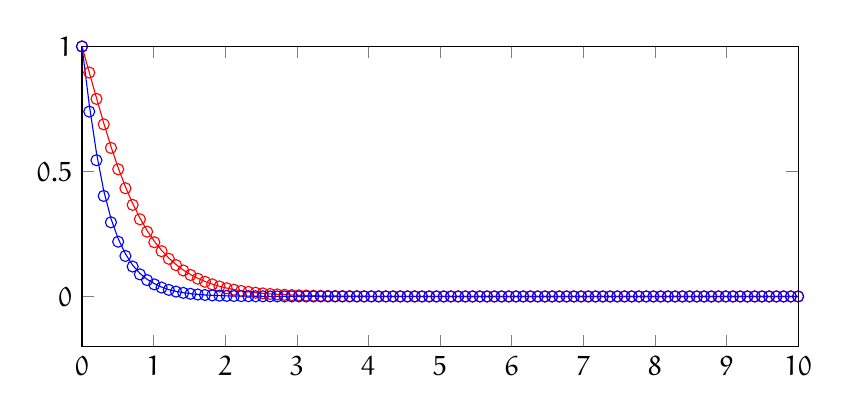
\begin{tikzpicture}

\begin{axis}[%
width=0.75\columnwidth,
height=1.5in,
at={(0.772in,0.473in)},
scale only axis,
xmin=0,
xmax=10,
ymin=-0.2,
ymax=1,
axis background/.style={fill=white}
]
\addplot [color=red, forget plot]
  table[row sep=crcr]{%
0	1\\
0.101010101010101	0.896423685753371\\
0.202020202020202	0.793659234448041\\
0.303030303030303	0.693944066226281\\
0.404040404040404	0.600137351677796\\
0.505050505050505	0.514729664848493\\
0.606060606060606	0.438794372885573\\
0.707070707070707	0.372001958315644\\
0.808080808080808	0.313663846287862\\
0.909090909090909	0.263376713743543\\
1.01010101010101	0.220640969080887\\
1.11111111111111	0.184447734417389\\
1.21212121212121	0.153659850476399\\
1.31313131313131	0.127572806294346\\
1.41414141414141	0.105792592254729\\
1.51515151515152	0.0877427992159511\\
1.61616161616162	0.0726424988227922\\
1.71717171717172	0.0599225353181231\\
1.81818181818182	0.0493539294526375\\
1.91919191919192	0.0407212813960692\\
2.02020202020202	0.0336158208305302\\
2.12121212121212	0.0276456890570014\\
2.22222222222222	0.0226574191448095\\
2.32323232323232	0.0186090412290333\\
2.42424242424242	0.0153413244276616\\
2.52525252525253	0.0126153165106946\\
2.62626262626263	0.0103070770928552\\
2.72727272727273	0.00842219544153099\\
2.82828282828283	0.00693201875250815\\
2.92929292929293	0.00571375330652814\\
3.03030303030303	0.00466713798360251\\
3.13131313131313	0.00379186278897362\\
3.23232323232323	0.00310850298118374\\
3.33333333333333	0.00257130550003406\\
3.43434343434343	0.00210883776325299\\
3.53535353535354	0.00170520617675866\\
3.63636363636364	0.00138647401322519\\
3.73737373737374	0.001149012333368\\
3.83838383838384	0.000951062203581647\\
3.93939393939394	0.000768791863445705\\
4.04040404040404	0.000617253233718878\\
4.14141414141414	0.000509257421419575\\
4.24242424242424	0.000427035814504569\\
4.34343434343434	0.000348274508720062\\
4.44444444444444	0.000275837964262336\\
4.54545454545455	0.000223921244895915\\
4.64646464646465	0.000189925799062625\\
4.74747474747475	0.000158342559326416\\
4.84848484848485	0.000124628006903808\\
4.94949494949495	9.81056469998393e-05\\
5.05050505050505	8.31292757043841e-05\\
5.15151515151515	7.17742597061688e-05\\
5.25252525252525	5.72578781561447e-05\\
5.35353535353535	4.3315047504837e-05\\
5.45454545454545	3.56419836185541e-05\\
5.55555555555556	3.20219292044079e-05\\
5.65656565656566	2.67198324995569e-05\\
5.75757575757576	1.96268173468927e-05\\
5.85858585858586	1.50222112168188e-05\\
5.95959595959596	1.38072992734395e-05\\
6.06060606060606	1.25027176976581e-05\\
6.16161616161616	9.28870252549169e-06\\
6.26262626262626	6.36254282619093e-06\\
6.36363636363636	5.63571533423865e-06\\
6.46464646464646	5.71225862997784e-06\\
6.56565656565657	4.59851873977577e-06\\
6.66666666666667	2.84345615532918e-06\\
6.76767676767677	2.14485625196088e-06\\
6.86868686868687	2.4464668021902e-06\\
6.96969696969697	2.32142713413607e-06\\
7.07070707070707	1.41841319761482e-06\\
7.17171717171717	7.75833753745334e-07\\
7.27272727272727	9.22488774128391e-07\\
7.37373737373737	1.13717998561667e-06\\
7.47474747474747	7.94224633060583e-07\\
7.57575757575758	3.04862016087248e-07\\
7.67676767676768	2.70092458069659e-07\\
7.77777777777778	5.03745161443354e-07\\
7.87878787878788	4.66966984167784e-07\\
7.97979797979798	1.67378538489673e-07\\
8.08080808080808	3.74590437161335e-08\\
8.18181818181818	1.77940967069056e-07\\
8.28282828282828	2.63007584523873e-07\\
8.38383838383838	1.26159762074514e-07\\
8.48484848484848	-1.42862946009757e-08\\
8.58585858585859	2.99022515559681e-08\\
8.68686868686869	1.29536068084732e-07\\
8.78787878787879	9.91266798592569e-08\\
8.88888888888889	-5.31633552370837e-09\\
8.98989898989899	-2.08987260250134e-08\\
9.09090909090909	4.81605562631398e-08\\
9.19191919191919	6.92552087690994e-08\\
9.29292929292929	1.17181111611164e-08\\
9.39393939393939	-2.58736527504535e-08\\
9.49494949494949	5.92934754376959e-09\\
9.5959595959596	4.02141144174707e-08\\
9.6969696969697	2.00804807791865e-08\\
9.7979797979798	-1.5257229708102e-08\\
9.8989898989899	-1.02341391865482e-08\\
10	1.76401286431667e-08\\
};
\addplot [color=blue, forget plot]
  table[row sep=crcr]{%
0	1\\
0.101010101010101	0.767441860465116\\
0.202020202020202	0.573969122532734\\
0.303030303030303	0.423185404790318\\
0.404040404040404	0.3118091703117\\
0.505050505050505	0.230844148159845\\
0.606060606060606	0.170579851385429\\
0.707070707070707	0.125238905341372\\
0.808080808080808	0.092233678200963\\
0.909090909090909	0.0687547231679837\\
1.01010101010101	0.0512424901386117\\
1.11111111111111	0.0375083437707221\\
1.21212121212121	0.027270540955226\\
1.31313131313131	0.0203064671625561\\
1.41414141414141	0.0153792063183289\\
1.51515151515152	0.0113169546382441\\
1.61616161616162	0.00804175569287034\\
1.71717171717172	0.00589365948240993\\
1.81818181818182	0.00459341118806526\\
1.91919191919192	0.00348771392516236\\
2.02020202020202	0.00240728317223041\\
2.12121212121212	0.00166046501901362\\
2.22222222222222	0.00133176859485923\\
2.32323232323232	0.00110299114058595\\
2.42424242424242	0.000759826528672681\\
2.52525252525253	0.000452480761477095\\
2.62626262626263	0.000351130099578734\\
2.72727272727273	0.000350103826784119\\
2.82828282828283	0.000267328723772301\\
2.92929292929293	0.000127211855966895\\
3.03030303030303	6.97168152364549e-05\\
3.13131313131313	0.000101508789054229\\
3.23232323232323	0.000106564702262825\\
3.33333333333333	4.65851881926789e-05\\
3.43434343434343	1.33035414487297e-06\\
3.53535353535354	1.84614041926607e-05\\
3.63636363636364	4.42901534331584e-05\\
3.73737373737374	2.6303550742097e-05\\
3.83838383838384	-6.58409180880169e-06\\
3.93939393939394	-6.14287849511743e-06\\
4.04040404040404	1.58822467230128e-05\\
4.14141414141414	1.77637317481637e-05\\
4.24242424242424	-1.67599691679939e-06\\
4.34343434343434	-9.68073823966168e-06\\
4.44444444444444	2.57094699636507e-06\\
4.54545454545455	1.10156510293878e-05\\
4.64646464646465	2.62546117993943e-06\\
4.74747474747475	-6.68137173700807e-06\\
4.84848484848485	-2.65893188272617e-06\\
4.94949494949495	5.4665844601414e-06\\
5.05050505050505	4.04784076177427e-06\\
5.15151515151515	-2.93087796075653e-06\\
5.25252525252525	-3.62669653633064e-06\\
5.35353535353535	1.68184219856028e-06\\
5.45454545454545	3.47825616287685e-06\\
5.55555555555556	-3.57842978620705e-07\\
5.65656565656566	-2.76541795773757e-06\\
5.75757575757576	-3.23561791049804e-07\\
5.85858585858586	2.17681713233273e-06\\
5.95959595959596	8.30723889340608e-07\\
6.06060606060606	-1.50295016811276e-06\\
6.16161616161616	-1.01034859533855e-06\\
6.26262626262626	9.65393859126222e-07\\
6.36363636363636	1.05382159002451e-06\\
6.46464646464646	-5.02374696635735e-07\\
6.56565656565657	-9.5717725737662e-07\\
6.66666666666667	1.70020052223553e-07\\
6.76767676767677	8.08134294015876e-07\\
6.86868686868687	6.54063634056825e-08\\
6.96969696969697	-6.26282195453777e-07\\
7.07070707070707	-2.04551953577808e-07\\
7.17171717171717	4.5001218068039e-07\\
7.27272727272727	2.74297276496859e-07\\
7.37373737373737	-2.90817927330253e-07\\
7.47474747474747	-2.89653841256182e-07\\
7.57575757575758	1.60997959592064e-07\\
7.67676767676768	2.70646206170755e-07\\
7.77777777777778	-6.17178601093467e-08\\
7.87878787878788	-2.30774719936341e-07\\
7.97979797979798	-7.37864420156827e-09\\
8.08080808080808	1.8221232494663e-07\\
8.18181818181818	5.06714647051537e-08\\
8.28282828282828	-1.32769531526282e-07\\
8.38383838383838	-7.29660619417098e-08\\
8.48484848484848	8.79382769460911e-08\\
8.58585858585859	7.97708209559664e-08\\
8.68686868686869	-5.05006371002456e-08\\
8.78787878787879	-7.59801842965636e-08\\
8.88888888888889	2.16051337405379e-08\\
8.98989898989899	6.58756405769482e-08\\
9.09090909090909	-1.0436597026223e-09\\
9.19191919191919	-5.27655825946432e-08\\
9.29292929292929	-1.21225728662176e-08\\
9.39393939393939	3.90858659157431e-08\\
9.49494949494949	1.926153092304e-08\\
9.5959595959596	-2.64264042186277e-08\\
9.6969696969697	-2.18423223716701e-08\\
9.7979797979798	1.57025088528739e-08\\
9.8989898989899	2.12671722736456e-08\\
10	-7.29477015521074e-09\\
};
\addplot [color=red, only marks, mark=o, mark options={solid, red}, forget plot]
  table[row sep=crcr]{%
0	1\\
0.101010101010101	0.895794706456733\\
0.202020202020202	0.790342927706555\\
0.303030303030303	0.68863344012746\\
0.404040404040404	0.594267368617498\\
0.505050505050505	0.508829040634649\\
0.606060606060606	0.43292841062441\\
0.707070707070707	0.366444791066423\\
0.808080808080808	0.308802319397216\\
0.909090909090909	0.259252890233671\\
1.01010101010101	0.216959099175846\\
1.11111111111111	0.181064890396212\\
1.21212121212121	0.150746890738321\\
1.31313131313131	0.125240933067143\\
1.41414141414141	0.103858251282719\\
1.51515151515152	0.0859874687348197\\
1.61616161616162	0.0710909095848059\\
1.71717171717172	0.058701279402423\\
1.81818181818182	0.0484166688053868\\
1.91919191919192	0.039894299554569\\
2.02020202020202	0.0328431972572441\\
2.12121212121212	0.0270173183986362\\
2.22222222222222	0.0222094579382915\\
2.32323232323232	0.0182458407865829\\
2.42424242424242	0.0149813006095828\\
2.52525252525253	0.0122949691215597\\
2.62626262626263	0.0100861358348373\\
2.72727272727273	0.00827096031142133\\
2.82828282828283	0.00678000644529375\\
2.92929292929293	0.00555598898164479\\
3.03030303030303	0.00455165172548003\\
3.13131313131313	0.00372794603760275\\
3.23232323232323	0.00305273258089904\\
3.33333333333333	0.00249934810208517\\
3.43434343434343	0.00204593063323589\\
3.53535353535354	0.00167452987652217\\
3.63636363636364	0.00137029128722434\\
3.73737373737374	0.00112115730121337\\
3.83838383838384	0.000917217266842587\\
3.93939393939394	0.000750307846490844\\
4.04040404040404	0.000613711820911806\\
4.14141414141414	0.000501943349722397\\
4.24242424242424	0.000410552016981992\\
4.34343434343434	0.000335767766532429\\
4.44444444444444	0.000274625880953453\\
4.54545454545455	0.000224593228982083\\
4.64646464646465	0.000183665269977384\\
4.74747474747475	0.000150192628063576\\
4.84848484848485	0.000122802133536067\\
4.94949494949495	0.000100411378783463\\
5.05050505050505	8.2095900915023e-05\\
5.15151515151515	6.71239667472742e-05\\
5.25252525252525	5.48836900847684e-05\\
5.35353535353535	4.48738837274167e-05\\
5.45454545454545	3.67221316313733e-05\\
5.55555555555556	3.00553270221419e-05\\
5.65656565656566	2.46149452164992e-05\\
5.75757575757576	2.01837749279476e-05\\
5.85858585858586	1.65348092113463e-05\\
5.95959595959596	1.3569909314629e-05\\
6.06060606060606	1.11236376647931e-05\\
6.16161616161616	9.11680650819259e-06\\
6.26262626262626	7.47024457135387e-06\\
6.36363636363636	6.11310043030165e-06\\
6.46464646464646	5.00397534290891e-06\\
6.56565656565657	4.09317118703542e-06\\
6.66666666666667	3.35287435304819e-06\\
6.76767676767677	2.74796773983367e-06\\
6.86868686868687	2.25292380751142e-06\\
6.96969696969697	1.85177121244251e-06\\
7.07070707070707	1.51780179884883e-06\\
7.17171717171717	1.23471148512651e-06\\
7.27272727272727	9.97932773883439e-07\\
7.37373737373737	8.03949522260452e-07\\
7.47474747474747	6.53670717978325e-07\\
7.57575757575758	5.10011214061725e-07\\
7.67676767676768	3.90248933743949e-07\\
7.77777777777778	2.97318671331267e-07\\
7.87878787878788	2.37306095857469e-07\\
7.97979797979798	1.75830091982791e-07\\
8.08080808080808	1.25710077350874e-07\\
8.18181818181818	9.07349100041773e-08\\
8.28282828282828	7.34223982265763e-08\\
8.38383838383838	5.78332026884001e-08\\
8.48484848484848	4.53607838997973e-08\\
8.58585858585859	3.76880492616666e-08\\
8.68686868686869	3.40142195366795e-08\\
8.78787878787879	3.17594529766311e-08\\
8.88888888888889	2.97887376392267e-08\\
8.98989898989899	2.77290621564245e-08\\
9.09090909090909	2.48642621011686e-08\\
9.19191919191919	2.1602566745788e-08\\
9.29292929292929	1.82586404201217e-08\\
9.39393939393939	1.4710039017142e-08\\
9.49494949494949	1.14176944861112e-08\\
9.5959595959596	7.86383316026895e-09\\
9.6969696969697	3.70273821818578e-09\\
9.7979797979798	1.39472389920266e-10\\
9.8989898989899	-2.16409878712879e-09\\
10	-2.40214119731233e-09\\
};
\addplot [color=blue, only marks, mark=o, mark options={solid, blue}, forget plot]
  table[row sep=crcr]{%
0	1\\
0.101010101010101	0.739446697718063\\
0.202020202020202	0.545048990201029\\
0.303030303030303	0.402140402819413\\
0.404040404040404	0.296698874715941\\
0.505050505050505	0.219118763888321\\
0.606060606060606	0.161918565713144\\
0.707070707070707	0.119621788471655\\
0.808080808080808	0.0883854845582368\\
0.909090909090909	0.0653128096623665\\
1.01010101010101	0.048254000614859\\
1.11111111111111	0.0356543521168761\\
1.21212121212121	0.026338977519388\\
1.31313131313131	0.0194521410709747\\
1.41414141414141	0.0143632396530483\\
1.51515151515152	0.0106066113465344\\
1.61616161616162	0.00783287758856351\\
1.71717171717172	0.00578361886370287\\
1.81818181818182	0.00426914766523074\\
1.91919191919192	0.00315098419149042\\
2.02020202020202	0.00232611727196387\\
2.12121212121212	0.00171750900163027\\
2.22222222222222	0.00126811960999498\\
2.32323232323232	0.000936172487785639\\
2.42424242424242	0.000691098525690028\\
2.52525252525253	0.000510381386746619\\
2.62626262626263	0.000377139224290743\\
2.72727272727273	0.000278721583348424\\
2.82828282828283	0.000205907718390331\\
2.92929292929293	0.00015206648376164\\
3.03030303030303	0.000112332695565052\\
3.13131313131313	8.3021635090115e-05\\
3.23232323232323	6.14298690081371e-05\\
3.33333333333333	4.54630222555316e-05\\
3.43434343434343	3.36466016942437e-05\\
3.53535353535354	2.48944319551014e-05\\
3.63636363636364	1.84021810580458e-05\\
3.73737373737374	1.36026982891067e-05\\
3.83838383838384	1.00650083829111e-05\\
3.93939393939394	7.45701975274642e-06\\
4.04040404040404	5.52388543936353e-06\\
4.14141414141414	4.08992915661415e-06\\
4.24242424242424	3.02771270005848e-06\\
4.34343434343434	2.23946889784436e-06\\
4.44444444444444	1.65869690633044e-06\\
4.54545454545455	1.23083143667391e-06\\
4.64646464646465	9.15274133692447e-07\\
4.74747474747475	6.83232984423311e-07\\
4.84848484848485	5.08574640412807e-07\\
4.94949494949495	3.78295765459602e-07\\
5.05050505050505	2.79860541916732e-07\\
5.15151515151515	2.06497919599185e-07\\
5.25252525252525	1.52567439846139e-07\\
5.35353535353535	1.13213571072638e-07\\
5.45454545454545	8.6784479936954e-08\\
5.55555555555556	6.73930983176342e-08\\
5.65656565656566	5.36032204686189e-08\\
5.75757575757576	4.42282218319026e-08\\
5.85858585858586	3.50053853402962e-08\\
5.95959595959596	2.81292313246194e-08\\
6.06060606060606	2.16930560110089e-08\\
6.16161616161616	1.57789972474467e-08\\
6.26262626262626	1.08990837896459e-08\\
6.36363636363636	7.49295170355875e-09\\
6.46464646464646	4.95421522341615e-09\\
6.56565656565657	3.4839019805376e-09\\
6.66666666666667	3.0244962051419e-09\\
6.76767676767677	2.88897999495319e-09\\
6.86868686868687	2.70755854796815e-09\\
6.96969696969697	2.7062015433171e-09\\
7.07070707070707	2.3660559999778e-09\\
7.17171717171717	2.59353408209182e-09\\
7.27272727272727	2.66863202015632e-09\\
7.37373737373737	2.44905131080726e-09\\
7.47474747474747	1.79724818133731e-09\\
7.57575757575758	1.35594349405689e-09\\
7.67676767676768	8.59646374139632e-10\\
7.77777777777778	3.90742394412667e-10\\
7.87878787878788	5.96678307865406e-11\\
7.97979797979798	-3.62900535293909e-10\\
8.08080808080808	-7.06782146417096e-10\\
8.18181818181818	-8.76466884377843e-10\\
8.28282828282828	-7.85682240747531e-10\\
8.38383838383838	-7.13588315953639e-10\\
8.48484848484848	-6.19521893440614e-10\\
8.58585858585859	-4.6931875740265e-10\\
8.68686868686869	-2.88409780347174e-10\\
8.78787878787879	-8.89197896155348e-11\\
8.88888888888889	9.87605758615117e-11\\
8.98989898989899	2.32661871385324e-10\\
9.09090909090909	2.70058711763343e-10\\
9.19191919191919	2.78667488503718e-10\\
9.29292929292929	2.91116088633421e-10\\
9.39393939393939	2.63894897124829e-10\\
9.49494949494949	1.99291475237685e-10\\
9.5959595959596	1.13645974965417e-10\\
9.6969696969697	2.63084411159642e-11\\
9.7979797979798	-5.35913894200833e-11\\
9.8989898989899	-1.0705032078714e-10\\
10	-1.11785729759658e-10\\
};
\end{axis}
\end{tikzpicture}%

\begin{itemize}
	\item[\faHammer]<4-> What can we say about the $A_m$ matrix?
\end{itemize}

\end{column}
\end{columns}

\end{frame}

\begin{frame}{Matrix properties}
$A_m$ is a banded Toeplitz matrix plus a rank correction.

\begin{columns}
\begin{column}{0.7\columnwidth}
\[
A_m = \begin{bmatrix}
	1 & \\
	-2 & \nicefrac{3}{2} \\
	\nicefrac{3}{2} & -3 & \nicefrac{11}{6} \\
	-\nicefrac{4}{3} & 3 & -4 & \nicefrac{25}{12} \\
	\nicefrac{5}{4} & -\nicefrac{10}{3} & 5 & -5 & \nicefrac{137}{60} \\
	-\nicefrac{6}{5} & \nicefrac{15}{4} & -\nicefrac{20}{3} & \nicefrac{15}{2} & -6 & \nicefrac{147}{60} \\
	\nicefrac{1}{6} & -\nicefrac{6}{5} & \nicefrac{15}{4} & -\nicefrac{20}{3} & \nicefrac{15}{2} & -6 & \nicefrac{147}{60} \\
	\vdots & \ddots & \ddots & \ddots & \ddots & \ddots & \ddots & \ddots \\
\end{bmatrix}
\]
\end{column}
\begin{column}{0.29\columnwidth}\centering
\only<2>{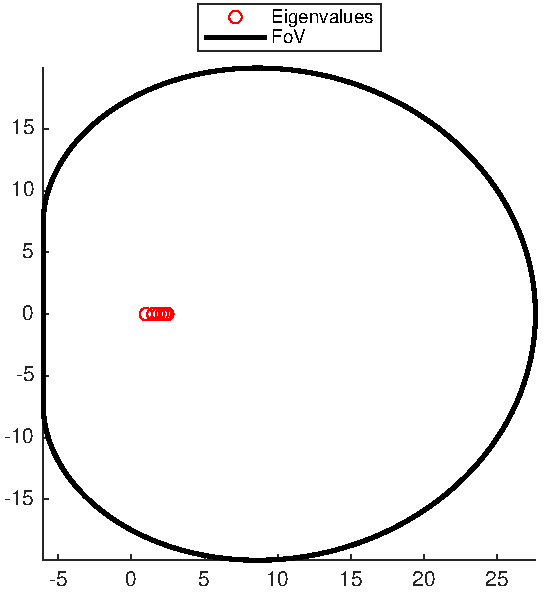
\includegraphics[width=0.9\columnwidth]{fov_m100.pdf}}%
\only<3>{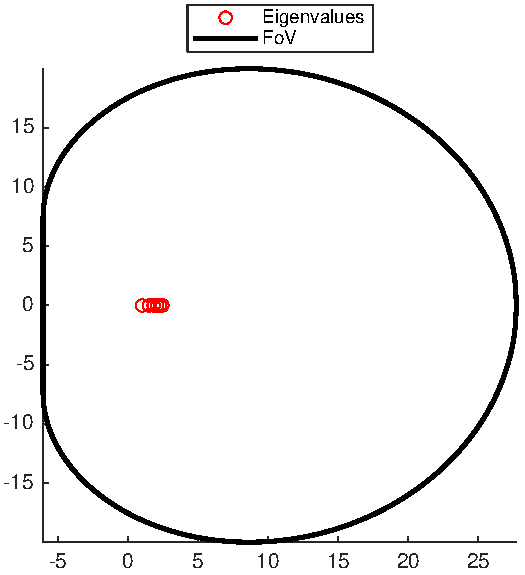
\includegraphics[width=0.9\columnwidth]{fov_m200.pdf}}%
\only<4>{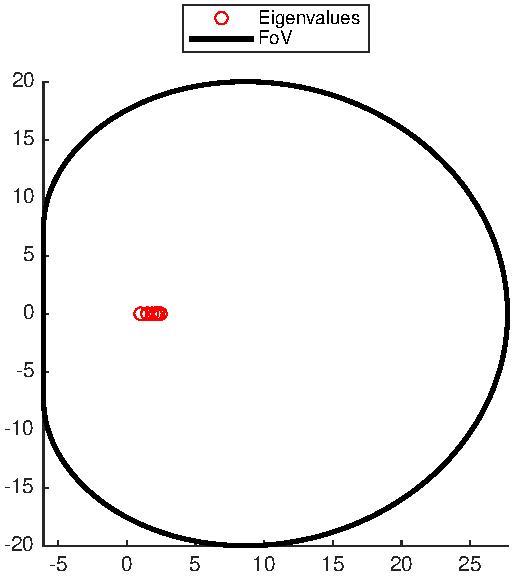
\includegraphics[width=0.9\columnwidth]{fov_m300.pdf}}%
\end{column}
\end{columns}
\begin{itemize}
	\item[\faCog] We know the eigenvalues in closed form: it's lower triangular!
	\item[\textcolor{Goldenrod}{\faSadTear}]<2-> The Field-Of-Values contains the origin$\ldots$ bad for bounds!
	\item[\alert{\faSadCry}]<4-> Its clearly \alert{non diagonalizable}, if we try and look at the condition number of the eigenvector matrix $\kappa_2(X_{100}) =  7.30 \times 10^{111}$. 
\end{itemize}
\end{frame}

\begin{frame}{Matrix properties}
Indeed, already for the BDF1 (a.k.a. the implicit Euler method) we have
\begin{columns}
\begin{column}{0.39\columnwidth}
\[
A_m = \begin{bmatrix}
	1 & \\
	-1 & 1 \\
	& \ddots & \ddots \\
	& & -1 & 1
\end{bmatrix}_{(m-1)\times(m-1)}
\]
\end{column}
\begin{column}{0.59\columnwidth}
\begin{itemize}
\item[\faCog] It is a Jordan block, so \emph{no diagonalization},
\item[\alert{\faQuestionCircle}]<2-> What do we expect for the matrix equation solver? \onslide<5>{ Nothing good!}
\end{itemize}
\end{column}
\end{columns}
\begin{columns}
\begin{column}{0.5\columnwidth}\only<3->{\small\centering
BDF1, $\alpha = 1.5$

\begin{tabular}{rrrl}
\toprule
$m$ & $n$ & IT & Residual \\
\midrule
%16 & 32 & 7 & 1.235969e-10  \\
%32 & 64 & 9 & 2.799035e-10  \\
64 & 128 & 13 & 1.007848e-10  \\
128 & 256 & 16 & 6.145733e-10  \\
256 & 512 & 21 & 7.639171e-10  \\
512 & 1024 & 27 & 5.857467e-10  \\
1024 & 2048 & 34 & 8.065585e-10  \\
2048 & 4096 & 42 & 9.819085e-10 \\
\bottomrule
\end{tabular}}
\end{column}
\begin{column}{0.5\columnwidth}\only<4->{\small\centering
BDF6, $\alpha = 1.5$

\begin{tabular}{rrrl}
	\toprule
	$m$ & $n$ & IT & Residual \\
	\midrule
%16 & 32 & 8 & 2.649653e-38 \\
%32 & 64 & 14 & 8.933887e-12 \\
64 & 128 & 21 & 3.651570e-10 \\
128 & 256 & 33 & 1.746513e-10 \\
256 & 512 & 71 & 2.530720e-15 \\
512 & 1024 & 128 & 1.975160e-22 \\
1024 & 2048 & 251 & 4.157259e-10 \\
2048 & 4096 & 495 & 6.310887e-10 \\
	\bottomrule
\end{tabular}}
\end{column}
\end{columns}

\end{frame}

\subsection{Linear Multistep Methods in Boundary Value Form}

\begin{frame}{Linear Multistep Methods in Boundary Value Form}
\faQuestionCircle\;Part of the problem, are those triangular matrices. Can we do something?
\vfill

\onslide<2->{\faHammer\; If we use \emph{more than one step}, we still need \textbf{auxiliary formulas} to close the iteration.\vfill}

\onslide<3->{\faLightbulb\; We could distribute the conditions differently, that is, not all on the initial data.

\[
\sum_{j=-\nu}^{\mu-\nu} \alpha_{j+\nu} \mathbf{u}_{n+j} =h
\sum_{j=-\nu}^{\mu-\nu} \beta_{j+\nu} \mathbf{f}_{n+j}, \quad n=\nu, \dots,
m-k+\nu.
\]
\begin{itemize}
	\item[\faPaperclip] $k$ steps,
	\item[\faPaperclip] $\nu$ initial conditions, and
	\item[\faPaperclip] $\mu-\nu$ final conditions,
	\item[\faPaperclip] Described by $\rho(z) = z^{\nu} \sum_{j=-\nu}^{k-\nu}\alpha_{j+\nu} z^j$, and $\sigma(z) = z^{\nu}\sum_{j=-\nu}^{k-\nu}\beta_{j+\nu} z^j$.
	\item[\faQuestionCircle]<4-> How does this change \alert{matrices} and \alert{stability}?
\end{itemize}
}

\end{frame}

\begin{frame}{Linear Multistep Methods in Boundary Value Form}
If we collect the matrices for the inner steps of a \emph{scalar} ODE, we get
\only<1>{\[\hspace{-1em}
A_m = \begin{bmatrix}
	\alpha_{\nu} & \cdots & \alpha_k \\
	\vdots & \ddots &  & \ddots \\
	\alpha_0 &  & \ddots & & \ddots \\
	& \ddots &  & \ddots & &\alpha_{k} \\
	& & \ddots &  &\ddots & \vdots \\
	& & & \alpha_0 & \cdots & \alpha_\nu 
\end{bmatrix}_{(m - \nu) \times (m-\nu)}\hspace{-2em}, B_m = \begin{bmatrix}
\beta_{\nu} & \cdots & \beta_k \\
\vdots & \ddots &  & \ddots \\
\beta_0 &  & \ddots & & \ddots \\
& \ddots &  & \ddots & &\beta_{k} \\
& & \ddots &  &\ddots & \vdots \\
& & & \beta_0 & \cdots & \beta_\nu 
\end{bmatrix}_{(m - \nu) \times (m-\nu)}
\]}\only<2->{ $A_m$, $B_m$,}
and the vectors
\[
\mathbf{u} = (u_{\nu},\cdots,u_{m-1})^T, \quad \mathbf{f} = (f_\nu,\cdots,f_{m-1})^T.
\]
\only<2->{Finding the system
\begin{columns}
\begin{column}{0.65\columnwidth}
\[
A_m \mathbf{u} - h B_m \mathbf{f} = - \begin{bmatrix}
	\sum_{j=0}^{\nu-1} (\alpha_j y_j - h \beta_j f_j) \\
	\vdots\\
	a_0 y_{\nu-1} - h \beta_0 f_{\nu-1} \\
	0 \\
	\vdots \\
	0 \\
	\alpha_k y_{m} - h \beta_k f_m \\
	\vdots \\
	\sum_{j=1}^{\mu} (\alpha_{\nu+j} y_{m-1+j} - h \beta_{\nu_1+j} f_{m-1+j}).
\end{bmatrix}
\]
\end{column}
\begin{column}{0.34\columnwidth}
\begin{itemize}
	\item[\faEye] $A_m$ and $B_m$ are Toeplitz matrices with \emph{lower bandwidth} $\nu$ and \emph{upper bandwidth} $\mu$.
	\item[\faHammer] We still need \alert{\textbf{auxiliary formulas}} to fix the $\nu+\mu-1$ starting/ending values.
\end{itemize}
\end{column}
\end{columns}
}
\end{frame}

\begin{frame}{Convergence and stability}
Before concluding the construction, let's focus on \emph{convergence} and \emph{stability}.

\onslide<2->{\faQuestionCircle\; Did we gain anything by moving on to a more difficult problem?}

\begin{block}<3->{$S_{\nu,\mu}$-polynomial \parencite[Definition 4.4.2]{MR1673796}}
A polynomial $p(z)$ of degree $k=\nu + \mu$ is an $S_{\nu,\mu}$-polynomial if its roots are such that
\[
|z_1| \leq |z_2| \leq \cdots \leq |z_{\nu}| < 1 < |z_{\nu+1}| \leq \cdots \leq |z_{\nu}|.
\]
\end{block}

\begin{block}<4->{$N_{\nu,\mu}$-polynomial \parencite[Definition 4.4.3]{MR1673796}}
	A polynomial $p(z)$ of degree $k=\nu + \mu$ is an $S_{\nu,\mu}$-polynomial if its roots are such that
	\[
	|z_1| \leq |z_2| \leq \cdots \leq |z_{\nu}| \leq 1 < |z_{\nu+1}| \leq \cdots \leq |z_{\nu}|.
	\]
	being \textbf{simple} the roots of unit modulus.
\end{block}

\onslide<5->{\alert{\faEye}\;If $\nu = k$ ($\mu = 0$), these are the conditions for LMF $0$-stability!}

\end{frame}

\begin{frame}{Convergence and stability}

\begin{columns}
\begin{column}{0.5\columnwidth}
Let $a_{-\nu}a_\mu \neq 0$ and 
\[
T_n = \begin{bmatrix}
	a_{0} & \cdots & a_{\mu} \\
	\vdots & \ddots &  & \ddots \\
	a_{-\nu} &  & \ddots & & \ddots \\
	& \ddots &  & \ddots & &a_{\mu} \\
	& & \ddots &  &\ddots & \vdots \\
	& & & a_{-\nu} & \cdots & a_0
\end{bmatrix},
\]
we consider the polynomial
\[
p(z) = \sum_{i=-\nu}^{\mu} a_i z^{\nu + i}.
\]
\end{column}
\begin{column}{0.5\columnwidth}\vspace{-1em}
\begin{alertblock}{Lemma~\parencite[Lemma 4.4.4]{MR1673796}}<2->
If the polynomial $p(z)$ associated with the matrix $T_n$ is an $N_{\nu,\mu}$-polynomial, then $T_n^{-1}$ has entries $t_{i,j}^{(-1)}$ such that
\begin{enumerate}
	\item $\lvert t_{i,j}^{(-1)} \rvert \leq \gamma $ independent of $N$, for $ i \geq j$,
	\item $\lvert t_{i,j}^{(-1)} \rvert \leq \eta \xi^{j-i}$ for $i < j$, where $\eta > 0$ and $0 < \xi < 1$ are independent of $N$.
\end{enumerate}
\end{alertblock}
\only<3->{\vspace{-1em}
\[
\text{\faEye}\;\lvert| T_n^{-1} \rvert| \leq \gamma C_n + \eta \Delta_n,
\]
with \only<3>{$C_n = \begin{bmatrix}
1 \\
\vdots & \ddots \\
1 & \cdots & 1
\end{bmatrix}$,}\only<4>{%
$\Delta_n$ the upper triangular Toeplitz matrix with last column
$(\xi^{n-1},\ldots,\xi^2,\xi,0)^T$.
} 
}
\end{column}
\end{columns}

\end{frame}

\begin{frame}{Convergence and stability}

\begin{alertblock}{Theorem~\parencite[Theorem 4.4.3]{MR1673796}}
Ignoring the effect of round-off errors, a BVM with $(\nu,\mu)$-boundary conditions is convergent if it is consistent and the polynomial $\rho(z)$ is an $N_{\nu,\mu}$-polynomial.
\end{alertblock}

\onslide<2->{To reproduce the ``$0$-stable $+$ consistent $\Rightarrow$ convergence'' framework, we define:}

\begin{block}<2->{$0_{\nu,\mu}$-stability~\parencite[Definition 4.5.1]{MR1673796}}
A BVM with $(\nu,\mu)$-boundary conditions is $0_{\nu,\mu}$-stable if the corresponding polynomial $\rho(z)$ is an $N_{\nu,\mu}$-polynomial.
\end{block}

\begin{block}<3->{$(\nu,\mu)$-Absolute stability~\parencite[Definition 4.7.1]{MR1673796}}
A BVM with $(\nu,\mu)$-boundary conditions is ${\nu,\mu}$-Absolutely stable for a given complex number $q$ it the polynomial $\pi(z,q) = \rho(z) - q \sigma(z)$, is an $S_{\nu,\mu}$-polynomial.
\end{block}

\end{frame}

\begin{frame}{Convergence and stability}
We have a degree of \alert{\textbf{arbitrariness}} in deciding how and how many initial / final conditions to set. Clearly $\nu$ has to be at least one (we do have an initial condition of our IVP), then for the remaining we have to let $(\nu,\mu)$-Absolute stability guide us.
\begin{description}
	\item[Correct use]<2-> a consistent LMF is \emph{correctly used} in $q \in \mathbb{C}^-$, where $\pi(z,q)$ is an $S_{\nu,\mu}$-polynomial, if $\nu$ conditions are imposed at the initial points, and $\mu$ conditions are posed at the end of the interval.
\end{description}

\onslide<3>{To have a livable life, one always consider family of methods for which the boundary of the  $(\nu,\mu)$-Absolutely stability region is a \emph{regular Jordan curve}. More specifically, having that
\[
\mathcal{A}_{\nu,\mu} = \{ q \in \mathbb{C}\,:\, \pi(z,q) \text{ is an } S_{\nu,\mu}\text{-polynomial} \},
\]
has the origin on its boundary and is possibly equal to the whole $\mathbb{C}^{-}$.}

\end{frame}

\begin{frame}{A gallery of formulas}

It is possible to reformulate many LMFs in this new format
\begin{itemize}
	\item[\faCog]<2-> BDF $\Rightarrow$ Generalized-BDF (GBDF): $\sum_{i=0}^{k} \alpha_i u_{n+i} = h f_{n+j}$, $j \in \{0,1,\ldots,k\}$
	 \begin{itemize}
	 	\item[\faExclamationCircle]<3-> \normalsize  A method of this form is $0_{\nu,k-\nu}$-stable and $A_{\nu,k-\nu}$-stable for
	 	\[
	 	\nu = \begin{cases}
	 		\frac{k+2}{2}, & \text{ for even }k,\\
	 		\frac{k+1}{2}, & \text{ for odd }k.
	 	\end{cases}
	 	\]
	 	$\Rightarrow$ with this choice we \alert{no longer have the constraint} of having at most $k=6$ steps of the standard BDF!
	 \end{itemize}
 	\item[\faCog]<3-> Adams-Moulton Methods $\Rightarrow$ GAMM $u_{n+j} - u_{n+j-1} = h \sum_{i=0}^{k} \beta_i f_{n+i}$
	 \begin{itemize}
 		\item[\faExclamationCircle]<4-> \normalsize  A method of this form is $0_{\nu,k-\nu}$-stable and $A_{\nu,k-\nu}$-stable for
 		\[
 		\nu = \begin{cases}
 			\frac{k+1}{2}, & \text{ for odd }k,\\
 			\frac{k}{2}, & \text{ for even }k.
 		\end{cases}
 		\]
 	\end{itemize}
 	\item[\faBook]<4-> See the book \parencite{MR1673796} for other possible generalizations.
\end{itemize}

\end{frame}

\subsection{Additional formulas}

\begin{frame}{Additional formulas}
\faHammer\;We need \textbf{additional formulas} for the $k-1=\nu+\mu-1$ boundary values.

\only<2>{
\begin{equation*}
	A_m = \begin{bmatrix}
		1 & \ldots & 0 \\
		\alpha_0^{(1)} & \ldots & \alpha_k^{(1)},\\
		\vdots & & \vdots \\
		\alpha_0^{(\nu-1)} & \ldots & \alpha_k^{(\nu-1)} \\
		\alpha_0 & \ldots & \alpha_k \\
		& \alpha_0 & \ldots & \alpha_k \\
		& & \ddots & \ddots & \ddots \\
		& & & \alpha_0 & \ldots & \alpha_k \\
		& & & \alpha_0^{(m-k+\nu+1)} & \ldots & \alpha_k^{(m-k+\nu+1)}\\
		& & & \vdots & & \vdots \\
		& & & \alpha_0^{(m)} & \ldots & \alpha_k^{(m)} \\
	\end{bmatrix},
\end{equation*}
}\only<3>{
\begin{equation*}
	B_m = \begin{bmatrix}
		0 & \ldots & 0 \\
		\beta_0^{(1)} & \ldots & \beta_k^{(1)},\\
		\vdots & & \vdots \\
		\beta_0^{(\nu-1)} & \ldots & \beta_k^{(\nu-1)} \\
		\beta_0 & \ldots & \beta_k \\
		& \beta_0 & \ldots & \beta_k \\
		& & \ddots & \ddots & \ddots \\
		& & & \beta_0 & \ldots & \beta_k \\
		& & & \beta_0^{(m-k+\nu+1)} & \ldots & \beta_k^{(m-k+\nu+1)},\\
		& & & \vdots & & \vdots \\
		& & & \beta_0^{(m)} & \ldots & \beta_k^{(m)} \\
	\end{bmatrix}.
\end{equation*}
}
\only<4->{
\begin{itemize}
	\item[\faCog] If we know how to compute them, then we end up having to solve the \textbf{matrix equation}
	\[
	M_n U A_m^T - h L_n U B_m^T = F,
	\]
	or the \textbf{linear system}
	\[
	(A_m \otimes M_n - h B_m \otimes L_n )\mathbf{u} = \mathbf{f}, \text{ where } \operatorname{vec}(U) = \mathbf{u}, \; \operatorname{vec}(F) = \mathbf{f}.
	\]
	\item[\faHammer]<5-> Let us build everything for using GBDFs and our fractional-in-space problem.
\end{itemize}
}


\end{frame}

\begin{frame}[fragile]{Generalized BDF}

\begin{columns}
\begin{column}{0.5\columnwidth}
First we need to compute $\rho(z)$ and $\sigma(z)$
\definecolor{bg}{rgb}{0.95,0.95,0.95}
\begin{minted}[bgcolor=bg,fontsize=\small,breaklines]{matlab}
function [ro,si] = rosi_bdf( k, j )
b  = zeros(k+1,1); b(2) = 1;
ro = vsolve( -j:k-j, b(:) );
si = zeros( k+1, 1 ); si( j+1 ) = 1;
end
\end{minted}
\vspace{-2em}\begin{itemize}
	\item[\faWrench] Coefficients are computed by \textbf{imposing consistency} of maximal order $p$:
	\[
	\sum_{j=0}^k(j^s \alpha_j - s j^{s-1} \beta_{j}) = 0,
	\]
	$s = 0,1,\ldots,p$.
\end{itemize}
\end{column}
\begin{column}{0.5\columnwidth}
\begin{onlyenv}<2->
\definecolor{bg}{rgb}{0.95,0.95,0.95}\vspace{-1em}
\begin{minted}[bgcolor=bg,fontsize=\small,breaklines]{matlab}
function f = vsolve( x, b )
f = b;
n = length( x )-1;
for k = 1:n
 for i = n+1:-1:k+1
  f(i) = f(i) - x(k)*f(i-1);
 end
end
for k = n:-1:1
 for i = k+1:n+1
  f(i) = f(i)/( x(i) - x(i-k) );
 end
 for i = k:n
  f(i) = f(i) - f(i+1);
 end
end
end
\end{minted}
\end{onlyenv}
\end{column}
\end{columns}

\end{frame}

\subsection{An example with GBDF}

\begin{frame}[fragile]{Generalized BDF}
Then we use the \mintinline{matlab}{ro_si} routine to build the $A_m$ and $B_m$ matrices
\begin{columns}
\begin{column}{0.5\columnwidth}
\definecolor{bg}{rgb}{0.95,0.95,0.95}\vspace{-1em}
\begin{minted}[bgcolor=bg,fontsize=\small,breaklines]{matlab}
function [a,b] = mab( k, n )
nu = fix( (k+2)/2 );
a  = spalloc( n, n+1, (k+1)*n );
b = a;
for i = 1:nu
 [ro,si] = rosi_bdf( k, i );
 a(i,1:k+1) = ro.';
 b(i,1:k+1) = si.';
end
for i = nu+1:n-(k-nu)
 a(i,i+1+(-nu:k-nu)) = ro.';
 b(i,i+1+(-nu:k-nu)) = si.';
end
\end{minted}
\end{column}
\begin{column}{0.5\columnwidth}
\definecolor{bg}{rgb}{0.95,0.95,0.95}\vspace{-1em}
\begin{minted}[bgcolor=bg,fontsize=\small,breaklines]{matlab}
j = nu;
for i = n-(k-nu)+1:n
 j = j + 1;
 [ro,si] = rosi_bdf( k, j );
 a(i,n+1+(-k:0)) = ro.';
 b(i,n+1+(-k:0)) = si.';
end
end
\end{minted}
\vspace{-2em}\begin{itemize}
	\item[\faCode] \mintinline{matlab}{for i = 1:nu; end}, initial conditions,
	\item[\faCode] \mintinline{matlab}{for i = nu+1:n-(k-nu); end}, Toepltiz part,
	\item[\faCode] \mintinline{matlab}{for i = n-(k-nu)+1:n; end}, final conditions.
\end{itemize}
\end{column}
\end{columns}
\end{frame}

\begin{frame}[fragile]{Generalized BDF}
We can use the routine to generate \mint{matlab}{[Alpha,Beta] = mab(k,m); A = Alpha(:,2:m+1); B = Beta(:,2:m+1);} and visualize them
\begin{center}
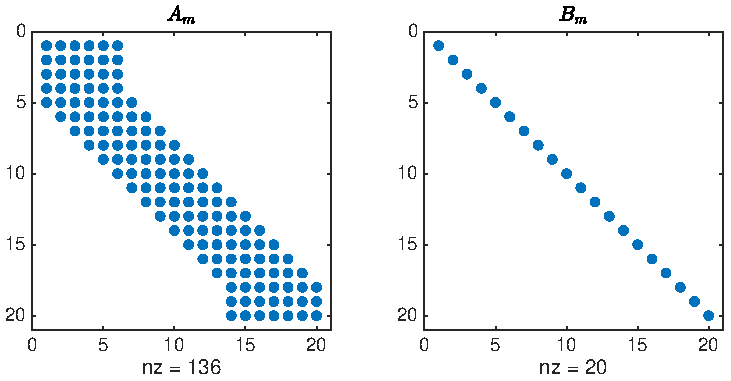
\includegraphics[width=0.6\columnwidth]{mab.pdf}
\end{center}
\faEye\;The first column contains the coefficients needed to compute the right-hand-side.
\end{frame}

\begin{frame}[fragile]{Generalized BDF}
We now need to build the right-hand-side\vspace{-0.7em}
\definecolor{bg}{rgb}{0.95,0.95,0.95}
\begin{minted}[bgcolor=bg,fontsize=\small,breaklines]{matlab}
nk=n*(m+1);
b=zeros(nk,1);  % Allocate the space for one more than needed
for j=1:m  % Use the source to build the rhs:
 b(1+j*n:(j+1)*n)=f(x,t0+j*h);
end 
b(n+1:n*(m+1))=h*kron(Beta,speye(n))*b; % Correct with the betas coeff.s
b(1:n)=u0; 		% First block as the initial condition
% Correction coefficients:
Am = kron(Alpha(:,1),speye(n))-h*kron(Beta(:,1),L);
b(n+1:nk)=b(n+1:nk)-Am*u0; % Finish building RHS
\end{minted}
And then we can solve the linear system\vspace{-0.7em}
\begin{minted}[bgcolor=bg,fontsize=\small,breaklines]{matlab}
Mat = kron(A,M) - h*kron(B,L); rhs = b(n+1:nk);
u = Mat\rhs;
\end{minted}
\end{frame}

\begin{frame}[fragile]{Generalized BDF}
We can compare the solution with \mintinline{matlab}{ode15s}:
\begin{onlyenv}<1>
\begin{columns}
\begin{column}{0.49\columnwidth}
\definecolor{bg}{rgb}{0.95,0.95,0.95}
\begin{minted}[bgcolor=bg,fontsize=\small,breaklines]{matlab}
U = [u0,reshape(u,n,m)]; t = t0:h:tf;
[TT,UU] = ode15s(@(t,y) L*y + f(x.',t),t,u0);
E = abs(U-reshape(UU,m+1,n).');
figure(2)
subplot(1,3,1)
mesh(t,x,U);
xlabel('t');
ylabel('x');
title('GBDF(6,100) on 100')
\end{minted}
\end{column}
\begin{column}{0.49\columnwidth}
\definecolor{bg}{rgb}{0.95,0.95,0.95}
\begin{minted}[bgcolor=bg,fontsize=\small,breaklines]{matlab}
subplot(1,3,2)
mesh(t,x,reshape(UU,m+1,n).')
xlabel('t');
ylabel('x');
title('ode15s')
subplot(1,3,3)
mesh(t,x,log10())
xlabel('t');
ylabel('x');
title('Error')
\end{minted}
\end{column}
\end{columns}
\end{onlyenv}
\only<2>{\begin{center}
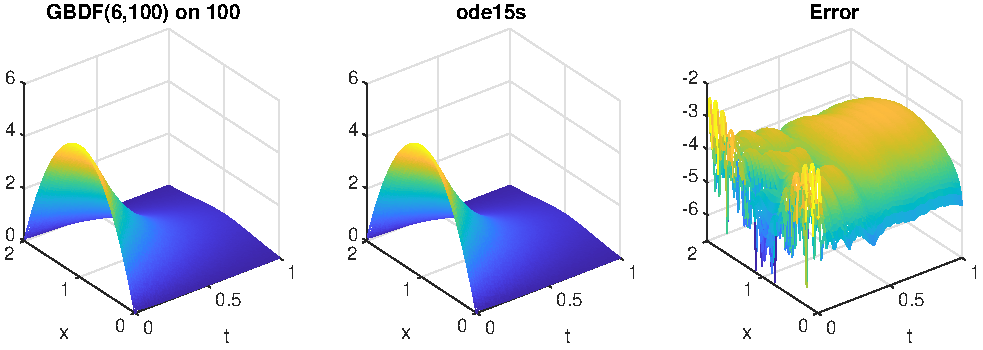
\includegraphics[width=0.8\columnwidth]{bvmsol.pdf}
\end{center}

\faQuestionCircle\; What happens if we attempt solution via our matrix-equation solver?
}

\end{frame}

\begin{frame}[fragile]{Generalized BDF}

\begin{columns}
\begin{column}{0.49\columnwidth}
We can solve it by doing:	
	
\definecolor{bg}{rgb}{0.95,0.95,0.95}
\begin{minted}[bgcolor=bg,fontsize=\small,breaklines]{matlab}
maxit = 100;
tol = 1e-9;
[LL,UL] = lu(-h*L);
[LA,UA] = lu(A);
[X1,X2,res]=kpik_sylv(-h*L,LL,UL,A, LA,UA,C1,C2,maxit,tol);
\end{minted}
Using our non-symmetric test problem with variable coefficients and fractional order $\alpha$.

\end{column}
\begin{column}{0.49\columnwidth}\centering
\begin{onlyenv}<2>
\begin{tabular}{crrrl}
\toprule
$k$ & $m$ & $n$ & IT & Res. \\
\midrule
2 & 32 & 64 & 16 & 1.08e-15\\
2 & 64 & 128 & 23 & 2.16e-10\\
2 & 128 & 256 & 30 & 4.72e-10\\
2 & 256 & 512 & 38 & 9.20e-10\\
2 & 512 & 1024 & 49 & 7.31e-10\\
2 & 1024 & 2048 & 62 & 7.82e-10\\
2 & 2048 & 4096 & 78 & 8.06e-10\\
2 & 4096 & 8192 & 97 & 9.24e-10\\
\bottomrule
\end{tabular}
\end{onlyenv}
\begin{onlyenv}<3>
	\begin{tabular}{crrrl}
		\toprule
		$k$ & $m$ & $n$ & IT & Res. \\
		\midrule
3 & 32 & 64 & 15 & 7.18e-10\\
3 & 64 & 128 & 20 & 9.80e-10\\
3 & 128 & 256 & 26 & 7.77e-10\\
3 & 256 & 512 & 34 & 4.21e-10\\
3 & 512 & 1024 & 43 & 5.75e-10\\
3 & 1024 & 2048 & 54 & 8.05e-10\\
3 & 2048 & 4096 & 68 & 8.84e-10\\
3 & 4096 & 8192 & 85 & 9.87e-10\\
		\bottomrule
	\end{tabular}
\end{onlyenv}
\begin{onlyenv}<4>
	\begin{tabular}{crrrl}
		\toprule
		$k$ & $m$ & $n$ & IT & Res. \\
		\midrule
4 & 32 & 64 & 16 & 1.19e-14\\
4 & 64 & 128 & 24 & 3.22e-10\\
4 & 128 & 256 & 31 & 4.05e-10\\
4 & 256 & 512 & 39 & 6.97e-10\\
4 & 512 & 1024 & 50 & 6.20e-10\\
4 & 1024 & 2048 & 63 & 7.70e-10\\
4 & 2048 & 4096 & 79 & 9.05e-10\\
4 & 4096 & 8192 & 99 & 9.05e-10\\
		\bottomrule
	\end{tabular}
\end{onlyenv}
\begin{onlyenv}<5>
	\begin{tabular}{crrrl}
		\toprule
		$k$ & $m$ & $n$ & IT & Res. \\
		\midrule
5 & 32 & 64 & 16 & 1.72e-14\\
5 & 64 & 128 & 22 & 2.96e-10\\
5 & 128 & 256 & 28 & 4.90e-10\\
5 & 256 & 512 & 36 & 5.56e-10\\
5 & 512 & 1024 & 46 & 5.53e-10\\
5 & 1024 & 2048 & 58 & 7.10e-10\\
5 & 2048 & 4096 & 73 & 8.04e-10\\
5 & 4096 & 8192 & 91 & 9.75e-10\\
		\bottomrule
	\end{tabular}
\end{onlyenv}
\begin{onlyenv}<6>
	\begin{tabular}{crrrl}
		\toprule
		$k$ & $m$ & $n$ & IT & Res. \\
		\midrule
6 & 32 & 64 & 16 & 3.46e-14\\
6 & 64 & 128 & 24 & 4.70e-10\\
6 & 128 & 256 & 31 & 5.73e-10\\
6 & 256 & 512 & 40 & 4.78e-10\\
6 & 512 & 1024 & 50 & 9.39e-10\\
6 & 1024 & 2048 & 64 & 7.69e-10\\
6 & 2048 & 4096 & 81 & 7.31e-10\\
6 & 4096 & 8192 & 100 & 1.10e-09\\
		\bottomrule
	\end{tabular}
\end{onlyenv}
\begin{onlyenv}<7>
	\begin{tabular}{crrrl}
		\toprule
		$k$ & $m$ & $n$ & IT & Res. \\
		\midrule
7 & 32 & 64 & 16 & 6.13e-15\\
7 & 64 & 128 & 22 & 6.60e-10\\
7 & 128 & 256 & 29 & 4.78e-10\\
7 & 256 & 512 & 37 & 7.04e-10\\
7 & 512 & 1024 & 47 & 8.47e-10\\
7 & 1024 & 2048 & 60 & 7.66e-10\\
7 & 2048 & 4096 & 76 & 7.36e-10\\
7 & 4096 & 8192 & 95 & 8.46e-10\\
		\bottomrule
	\end{tabular}
\end{onlyenv}
\begin{onlyenv}<8->
	\begin{tabular}{crrrl}
		\toprule
		$k$ & $m$ & $n$ & IT & Res. \\
		\midrule
8 & 32 & 64 & 16 & 2.46e-14\\
8 & 64 & 128 & 24 & 5.41e-10\\
8 & 128 & 256 & 31 & 7.57e-10\\
8 & 256 & 512 & 40 & 6.53e-10\\
8 & 512 & 1024 & 51 & 7.34e-10\\
8 & 1024 & 2048 & 65 & 6.98e-10\\
8 & 2048 & 4096 & 82 & 7.42e-10\\
8 & 4096 & 8192 & 100 & 1.56e-09\\
		\bottomrule
	\end{tabular}
\end{onlyenv}
\end{column}
\end{columns}
\vfill

\begin{itemize}
	\item[\faEye]<9-> The solution seems to be robust with respect to $k$,
	\item[\faEye]<10-> We still have a small increase with $n$ and $m$.
\end{itemize}
\end{frame}

\subsection{Structured preconditioner}

\begin{frame}[fragile]{Structured preconditioner}

Let's now look for a different approach.
\begin{itemize}
	\item[\faFastForward]<2-> We can do matrix vector products with the system matrix without assembling the matrix:\vspace{-1em}
	\definecolor{bg}{rgb}{0.95,0.95,0.95}
	\begin{minted}[bgcolor=bg,fontsize=\small,breaklines]{matlab}
function [y] = Mprod(A,B,L,h,x)
[sp1,~] = size(A);
[m,~] = size(L);
X = reshape(x,m,sp1);
Y = X*A' - h*(L*X*B');
y = reshape(Y,m*sp1,1);
end
	\end{minted}
	\item[\faWrench]<3-> The linear system is \alert{\textbf{not symmetric}}: we can use either GMRES or Flexible-GMRES to solve it.
	\item[\faHammer]<4-> We just need to \emph{figure out} a \emph{preconditioner}.
\end{itemize}

\end{frame}

\begin{frame}{Structured preconditioner}
The \alert{\faKey\,idea} is \emph{again} using a preconditioner that has the same structure:
\[
P = \breve{A}_m \otimes M_n -h \breve{B}_m \otimes \tilde{L}_n,
\]
\begin{itemize}
	\item[\faBook]<1-> This idea comes from~\parencite{MR1784824,MR1854266,MR1812028},
	\item[\faLightbulb]<2-> How do we select the approximations $\breve{A}_m$, $\breve{B}_m$ and $\tilde{L}_n$?
	\begin{itemize}
		\item[\faCog]<3-> \normalsize $A_m$, $B_m$ are Toeplitz + low-rank $\Rightarrow$ Circulant or Fast-Transform preconditioners,
		\item[\faCog]<3-> \normalsize $\tilde{L}_n$ has the \emph{quasi-Toeplitz structure} we have seen, so we can use some of the techniques we had already seen for this; \parencite{MR3860196}. 
	\end{itemize}
	\item[\faHammer]<4-> It would be good to also have a \alert{\textbf{parallel way of applying the preconditioner}}.
\end{itemize}
\end{frame}

\begin{frame}{Structured preconditioner}

\begin{itemize}
	\item[\faLightbulb] If $\breve{A}_m$ and $\breve{B}_m$ are \emph{circulant--like approximations} of the Toeplitz (+ ``low rank'') matrices $A_m$ and $B_m$, and the mass matrix is the identity, then we can express the \textbf{eigenvalues} of $P$ as
	\begin{equation*}
		\phi_i - h \psi_i \lambda_j, \qquad i = 1,\ldots,m, \quad j=1,\ldots,n,
	\end{equation*}
	where
	\begin{itemize}
		\item[\faWrench]\normalsize $\{\phi_i\}$ are the eigenvalues of the circulant--like approximation
		$\breve{A}$,
		\item[\faWrench]\normalsize $\{\psi_i\}$ are the eigenvalues of the circulant--like approximation $\breve{B}$,
		\item[\faWrench]\normalsize $\{\lambda_j\}$ are the eigenvalues of
		the selected approximation of $J_n$.
	\end{itemize}
	\item[\faQuestionCircle]<2-> What circulant-like approximation do we want?
	\begin{itemize}
		\item[\faCog]<3-> An idea could be using Strang approximation~\parencite{MR3272165}
		\[
		P_\mathfrak{s} = \mathfrak{s}(A_m)\otimes I_m - h \mathfrak{s}(B_m)\otimes L_n,
		\]
	\end{itemize}
\end{itemize}
                                                                                                                                                                        
\end{frame}

\begin{frame}{Structured preconditioner}
\[
\only<1-2>{P_\mathfrak{s} = \mathfrak{s}(A_m)\otimes I_m - h \mathfrak{s}(B_m)\otimes L_n,}%
\only<3->{P_{\tilde{\mathfrak{s}}} = \tilde{\mathfrak{s}}(A)_m\otimes I_n - h \tilde{\mathfrak{s}}(B)_m\otimes L_n.}
\]
\vspace{-2em}\begin{columns}
\begin{column}{0.7\columnwidth}
\[
\mathfrak{s}(A) = \begin{bmatrix} \alpha_{\nu} &\cdots &\alpha_k &
	&      &
	&\alpha_0 &\cdots &\alpha_{\nu-1}\\
	\vdots &    \ddots         &   &    \ddots   &   & &              &
	\ddots &   \vdots  \\
	\alpha_0 &         &   \ddots     & & \ddots &     &    &  & \alpha_0 \\
	& \ddots & &  \ddots      & &\ddots  &        &  0 &   \\
	&   & \ddots   &         & \ddots & & \ddots    &        \\
	& 0      &        & \ddots & &  \ddots & & \ddots  &    \\
	\alpha_k &         & &            & \ddots & & \ddots & &  \alpha_k \\
	\vdots & \ddots       &  & & & \ddots &  & \ddots & \vdots \\
	\alpha_{\nu+1}&\cdots  & \alpha_k &   & &        &  \alpha_0 &
	\cdots &  \alpha_{\nu}
\end{bmatrix},
\]
\end{column}
\begin{column}{0.3\columnwidth}
\begin{onlyenv}<1-3>
\begin{itemize}
	\item[\faCog] $\mathfrak{s}(B)$ can be built analogously.
	\item[\faSadTear]<2-> $\mathfrak{s}(A)$ is singular due to the consistency condition.
	\item[\faHammer]<3-> It is a single $0$ eigenvalue, so we can move it by a rank 1 perturbation: $\tilde{\mathfrak{s}}(\cdot)$.
\end{itemize}
\end{onlyenv}
\begin{onlyenv}<4>
\begin{alertblock}{Proposition \parencite[Proposition 4.1]{MR1812028}}
If $L$ has eigenvalues $\mu_r$ such that $\Re(\mu_r)  < -\delta < 0$, $r=1,\ldots,m$. Then the preconditioner $P_{\tilde{\mathfrak{s}}}$ is invertible for $A_{\nu,k-\nu}$-stable formulae.
\end{alertblock}
\end{onlyenv}
\end{column}
\end{columns}
\end{frame}

\begin{frame}{Structured preconditioner}
\alert{\faQuestionCircle}\;What can we say about the \alert{\textbf{clustering properties}} of this preconditioner?

\begin{alertblock}{Theorem~\parencite[Theorem~4.1]{MR1784824}}
Let $\mathcal{M} = A_m \otimes I_n - h B_m \otimes L_n$ for an $A_{\nu,k-\nu}$-stable formulae with $k$ steps. Let $P$ be the block circulant preconditioner
\[
P = \breve{A}_m \otimes M_n -h \breve{B}_m \otimes L_n.
\]
Then, for fixed $\delta > 0$, there exists $C_\delta \geq 0$, $m_\delta \geq k$ such that, for all $m \geq m_\delta$ ($m+1$ is the size of $A$ and $B$),
\[
P^{-1} M = I + M_\delta^{(1)} + M_{\delta}^{(2)},
\] 
where $\operatorname{rank}(M_\delta^{(2)}) \leq n[2(k+1) + C_\delta]$ and $\| M_\delta^{(1)}\|_2 \leq \delta c_L$ does not depend on $m$. If $P$ is defined as Strang's circulant preconditioner, then $C_\delta = \| M_\delta^{(1)}\| = 0$.
\end{alertblock}

\end{frame}

\begin{frame}{Structured preconditioner}

Another available choice is using instead $\{\omega\}$-Circulant matrices, i.e.,
\[
P_\omega = \omega(A_m)\otimes I_n - h \omega(B_m)\otimes L_n,
\]
\vspace{-2em}\begin{columns}
\begin{column}{0.7\columnwidth}\small
\[
\omega(A_m) =\begin{bmatrix} \alpha_{\nu} &\cdots &\alpha_k &   &
	&
	&\omega\alpha_0 &\cdots &\omega\alpha_{\nu-1}\\
	\vdots &    \ddots         &   &    \ddots   &   & &              &
	\ddots &   \vdots  \\
	\alpha_0 &         &   \ddots     & & \ddots &     &    &  & \omega\alpha_0 \\
	& \ddots & &  \ddots      & &\ddots  &        &  0 &   \\
	&   & \ddots   &         & \ddots & & \ddots    &        \\
	& 0 &        & \ddots & &  \ddots & & \ddots  &    \\
	\omega\alpha_k &         & &            & \ddots & & \ddots & &  \alpha_k \\
	\vdots & \ddots       &  & & & \ddots &  & \ddots & \vdots \\
	\omega\alpha_{\nu+1}&\cdots  & \omega\alpha_k &   & &        &
	\alpha_0 & \cdots &  \alpha_{\nu}
\end{bmatrix},
\]
\end{column}
\begin{column}{0.3\columnwidth}
\begin{itemize}
	\item[\faCog] $\omega(B_m)$ is defined similarly.
	\item[\faHammer] The usual choice is setting $\omega = -1$, i.e., the skew-circulant preconditioner.
\end{itemize}
\end{column}
\end{columns}
\end{frame}

\begin{frame}{Stuctured preconditioner: application}
	To apply 
	\[
	P_\omega^{-1} \mathbf{v} = (\omega(A_m)\otimes I_n - h \omega(B_m)\otimes L_n)^{-1}\mathbf{v},
	\]
	We can use the \textbf{diagonalization} of $\omega(A_m)$ and $\omega(B_m)$, i.e.,
	\[
	P_\omega^{-1} \mathbf{v} = (F\Omega \otimes I_n)^{-1} (\Lambda_A \otimes I_n - h \Lambda_B \otimes L_n)^{-1} (\Omega^{H}F^{H}\otimes I_n)^{-1} \mathbf{v}.
	\]
	\begin{enumerate}
		\item Compute $\mathbf{w} = (\Omega^{*}F^{*}\otimes I_m)^{-1} \mathbf{v} = - V \Omega^{-H}F$,
		\item Solve $(\Lambda_A \otimes I_n - h \Lambda_B \otimes L_n)^{-1} \mathbf{w}$ by solving
		\[
		\alert<2>{(\lambda_i(A) I_n - h \lambda_i(B) L_n) \mathbf{z}_i = \mathbf{w}_i, \quad i=1,\ldots,m}
		\]
		with $\operatorname{vec}([\mathbf{w}_1,\ldots,\mathbf{w}_m]) = \mathbf{w}$, and similarly for $\textbf{z}$,
		\item Compute $\mathbf{y} = (F\Omega \otimes I_n)^{-1} \mathbf{z} =  -Z F^H \Omega^{-1}$.
	\end{enumerate}

	\onslide<2>{\faExclamationCircle\; This step is \textbf{embarrassingly parallel}!}
\end{frame}

\begin{frame}{Numerical example}

We use our favorite test problem with the space variant, nonsymmetric fractional operator in space and $\alpha=1.5$, using GMRES(20) with a tolerance of \mintinline{matlab}{1e-9} using the $P_{-1}$ preconditioner.

\begin{columns}
\begin{column}{0.19\columnwidth}
\begin{tabular}{rrl}
\toprule
\multicolumn{3}{c}{$k=2$} \\
\midrule 
n & m & It \\
\midrule 
64 & 32 & 30 \\
128 & 64 & 31 \\
256 & 128 & 31 \\
512 & 256 & 31 \\
1024 & 512 & 30 \\
\bottomrule
\end{tabular}
\end{column}
\begin{column}{0.19\columnwidth}
\begin{tabular}{rrl}
	\toprule
	\multicolumn{3}{c}{$k=3$} \\
	\midrule 
	n & m & It \\
	\midrule 	
64 & 32 & 32 \\
128 & 64 & 33 \\
256 & 128 & 34 \\
512 & 256 & 34 \\
1024 & 512 & 33 \\
\bottomrule
\end{tabular}
\end{column}
\begin{column}{0.19\columnwidth}
\begin{tabular}{rrl}
	\toprule
	\multicolumn{3}{c}{$k=4$} \\
	\midrule 
	n & m & It \\
	\midrule 	
64 & 32 & 35 \\
128 & 64 & 38 \\
256 & 128 & 39 \\
512 & 256 & 39  \\
1024 & 512 & 37 \\
\bottomrule
\end{tabular}
\end{column}
\begin{column}{0.19\columnwidth}
\begin{tabular}{rrl}
	\toprule
	\multicolumn{3}{c}{$k=5$} \\
	\midrule 
	n & m & It \\
	\midrule 	
64 & 32 & 38 \\
128 & 64 & 45 \\
256 & 128 & 48 \\
512 & 256 & 50 \\
1024 & 512 & 49 \\
\bottomrule
\end{tabular}
\end{column}
\begin{column}{0.19\columnwidth}
\begin{tabular}{rrl}
	\toprule
	\multicolumn{3}{c}{$k=6$} \\
	\midrule 
	n & m & It \\
	\midrule 
64 & 32 & 46 \\
128 & 64 & 53 \\
256 & 128 & 58 \\
512 & 256 & 62 \\
1024 & 512 & 60 \\
\bottomrule
\end{tabular}
\end{column}
\end{columns}
\vfill

\onslide<2>{\definecolor{success}{HTML}{4a934a}\faEye\;Reduced \textcolor{success}{\faSmile\;\textbf{iteration dependence}}, but paid with \alert{\faSadTear\;\textbf{full memory price}}!}

\end{frame}

\begin{frame}{Further modifications}
We can further approximate the preconditioner by selecting instead of $L_n$ in
\[
P_\omega^{-1} \mathbf{v} = (\omega(A_m)\otimes I_n - h \omega(B_m)\otimes L_n)^{-1}\mathbf{v},
\]
a suitable approximation, e.g.,
\begin{itemize}
	\item[\faCog] $g_k(L_n)$ a bandwidth $k$ approximation of the dense $L_n$ matrix, i.e., using the information on the decay of the coefficients~\parencite{MR3860196}.
	\item[\faCog] A \emph{structured preconditioner} based on GLT theory.
\end{itemize}

\begin{exampleblock}<2->{\faBinoculars\; Open areas of research}
\begin{itemize}
	\item[\faWalking] Efficient solution strategies for the $\lambda_i(A) I_n - h \lambda_i(B) L_n$ systems,
	\item[\faWalking] Load-balancing issues for parallelism, 
	\item[\faWalking] Optimal poles selection for the matrix-equation based solvers,
	\item[\faWalking] Multigrid solvers/preconditioners for $({A_m} \otimes M_n - h {B_m} \otimes L_n) \mathbf{u} = {\mathbf{f}}$.
\end{itemize}
\end{exampleblock}

\end{frame}

\subsection{Tensor Equations}

\begin{frame}{\faCompress\;Tensor Equations}

\faHammer\;A \emph{different approach} that can be of interest is to use \alert{another structure}.\vfill

\onslide<2->{\faLightbulb\;Let us suppose that $L_n$ is obtained as the discretization of a \emph{multidimensional fractional operator}, i.e.,
\[
L_n = \sum_{i=1}^{\ell} \left(K_{m,\ell}^{-} \bigotimes_{p=1}^{i-1} I \otimes G_{n^{1/\ell}}^{(\ell)} \otimes \bigotimes_{p=1}^{\ell-1} I + K_{n,\ell}^{+}\bigotimes_{p=1}^{i-1} I \otimes {G_{n^{1/\ell}}^{(\ell)}}^T \otimes \bigotimes_{p=1}^{\ell-1} I\right)
\]
where $K_{m,\ell}^{\pm}$ have also a Kronecker tensor structure whenever the functions $\{\kappa_j\}_{j=1}^{\ell}$ are separable in the $x_j$ variables.\vfill
}

\onslide<3->{
The matrix:
$\mathcal{M} = A_m\otimes I_n - h  B_m \otimes L_n$ has now a lot of \alert{\textbf{redundant information}}!
}

\end{frame}

\begin{frame}{\faCompress\;Tensor Equations: \emph{thou shalt compress}!}

As we have done for the \emph{hierarchical formats}, we want
\begin{itemize}
	\item[\faGem] A \alert{\textbf{compressed representation}} of $\mathcal{M}$, possibly with a number of parameters that grows poly-logarithmically with the overall size$\ldots$
	\item[\faToolbox] A \alert{\textbf{fast BLAS-like toolbox}} to solve our problem in this format.
\end{itemize}
\vfill

\onslide<2->{There exists \emph{many formats} for which this is possible, \emph{e.g.}, the CANDECOMP/PARAFAC (CP) decomposition, the Tucker format, the \alert<3>{Tensor Train} (TT), the TT-Tucker, \emph{etc.}; see \parencite{MR2535056}.\vfill}

\onslide<3>{We focus on the \faTrain\;\alert{\textbf{T}}ensor-\alert{\textbf{T}}rain format, since it has a simple enough toolbox to work with: \href{https://github.com/oseledets/TT-Toolbox}{\faGithub\; TT-Toolbox}.}

\end{frame}

\begin{frame}{\faTrain\;Tensor-Train}
\faQuestionCircle\;But what is a \emph{tensor}?

\begin{itemize}
	\item[\faBook]<2-> A \textbf{tensor} is a \textbf{multidimensional array}, $a \in \mathbb{R}$ is a 0-tensor, $\mathbf{v} \in \mathbb{R}^{n_1}$ is a 1-tensor, $A \in \mathbb{R}^{{n_1} \times {n_2}}$ is a 2-tensor, $\mathbf{\mathcal{A}} \in \mathbb{R}^{{n}_1 \times n_{2} \times n_3}$ is a 3-tensor, $\ldots$
	\item[\faBook]<3-> A \textbf{tensor} is a \textbf{multilinear maps} with respect to a fixed finite-dimensional $\mathbb{R}$ vector space $V$
	\[
	\mathbf{\mathcal{A}} \,: \underbrace{V^* \times \cdots \times V^*}_p \times \underbrace{V \times \cdots \times V}_q \rightarrow \mathbb{R},
	\]
	\item[\faBook]<4-> A \textbf{tensor} is an \textbf{element of the tensor product} of vector spaces
	\[
	\mathbf{\mathcal{A}} \in \underbrace{V \times \cdots \times V}_p \otimes \underbrace{V^* \otimes \cdots \otimes V^*}_q.
	\]
\end{itemize}

\onslide<5>{The definition we select depends on the operations we want to perform.}

\end{frame}

\begin{frame}{\faTrain\;Tensor-Train\footnotemark}
Let us start from trying to describe a \emph{vector} associated with our discretization matrix $\mathcal{M}$.

\onslide<2->{\faLightbulb\;A rank-$k$ matrix $A=U_1U_2^T$ each entry is a dot product of vectors of length $k$ 
\begin{center}
	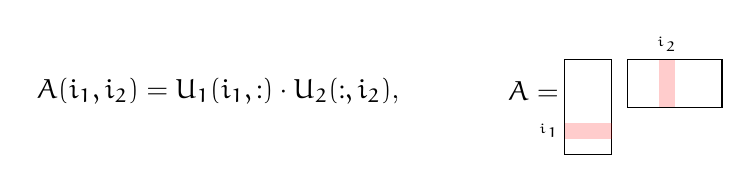
\begin{tikzpicture}[scale=.2]
		\node at (0,-2){$A=$};
		\node at (1,-4.5){\tiny $i_1$};
		\node at (8.5,1){\tiny $i_2$};
		\draw (2,0) rectangle (5,-6);
		\draw (6,0) rectangle (12,-3);
		\fill[red,opacity=0.2] (2,-4) rectangle (5,-5);
		\fill[red,opacity=0.2] (8,0) rectangle (9,-3);
		\node at (-20,-2){	$
			A(i_1,i_2)= U_1(i_1,:) \cdot U_2(:, i_2)
			$,};
	\end{tikzpicture}
\end{center}
where the two indices select the left and right vectors.}
\onslide<3>{
In a \alert{tensor of order $d$} we insert $d-2$ matrices between the two vectors:
$$
\mathcal T(i_1,\dots,i_d)= U_1(i_1,\ :)\cdot U_2(:,\ :,\ i_2)\cdot\ \dots \ \cdot U_{d-1}(:,\ :,\ i_{d-1})\cdot U_d(:,\ i_d)
$$
\begin{center}
	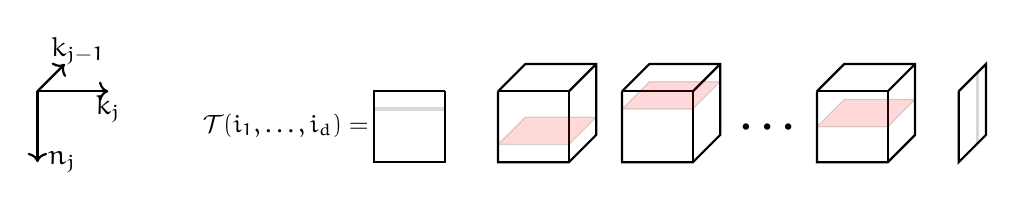
\begin{tikzpicture}[scale=.9]
		\draw[thick](0,2,1)--(0,2,0)--(1,2,0)--(1,1,0)--(1,1,1)--(0,1,1)--(0,2,1);
		\draw[thick](0,2,1)--(1,2,1)--(1,1,1);
		\draw[thick] (1,2,1)--(1,2,0);
		\draw[thick](1.75,2,1)--(1.75,2,0)--(2.75,2,0)--(2.75,1,0)--(2.75,1,1)--(1.75,1,1)--(1.75,2,1);
		\draw[thick](1.75,2,1)--(2.75,2,1)--(2.75,1,1);
		\draw[thick] (2.75,2,1)--(2.75,2,0);
		\node at (3.85,1.5, 1) {\begin{LARGE}$\dots$\end{LARGE}};		
		\draw[thick](4.5,2,1)--(4.5,2,0)--(5.5,2,0)--(5.5,1,0)--(5.5,1,1)--(4.5,1,1)--(4.5,2,1);
		\draw[thick](4.5,2,1)--(5.5,2,1)--(5.5,1,1);
		\draw[thick] (5.5,2,1)--(5.5,2,0);
		\draw[thick] (-.75,2,1)--(-1.75,2,1)--(-1.75,1,1)--(-.75,1,1)--(-.75,2,1);
		\draw[thick] (6.5,2,1)--(6.5,2,0)--(6.5,1,0)--(6.5,1,1)--(6.5,2,1);
		\draw[->,thick] (-6.5,2,1)--(-6.5,2,0);
		\draw[->,thick] (-6.5,2,1)--(-6.5,1,1);
		\draw[->,thick] (-6.5,2,1)--(-5.5,2,1);
		\node at (-6.15,1,1){$n_j$};
		\node at (-5.5,1.75,1){$k_{j}$};
		\node at (-6.5,2,-.5){$k_{j-1}$};
		\node at (-3,1.5, 1) {\begin{small}$\mathcal T(i_1,\dots,i_d)=$\end{small}};
		
		\draw[very thick,fill=red,opacity=.15](-1.75,1.75,1)--(-0.75,1.75,1);
		\draw[fill=red,opacity=.15](0,1.25,1)--(1,1.25,1)--(1,1.25,0)--(0,1.25,0)--(0,1.25,1);
		\draw[fill=red,opacity=.15](1.75,1.75,1)--(2.75,1.75,1)--(2.75,1.75,0)--(1.75,1.75,0)--(1.75,1.75,1);
		\draw[fill=red,opacity=.15](4.5,1.5,1)--(5.5,1.5,1)--(5.5,1.5,0)--(4.5,1.5,0)--(4.5,1.5,1);
		\draw[very thick,fill=red,opacity=.15] (6.5,2,.3)--(6.5,1,.3);
	\end{tikzpicture}
\end{center}
}
\footnotetext[1]{For part of this material, a sincere thanks to Stefano Massei.}
\end{frame}

\begin{frame}{\faTrain\;Tensor-Train}
More formally, a tensor $\mathcal T$ is in \alert{TT decomposition} if it can be written as%
	\begin{onlyenv}<1>%
		\begin{center}%
		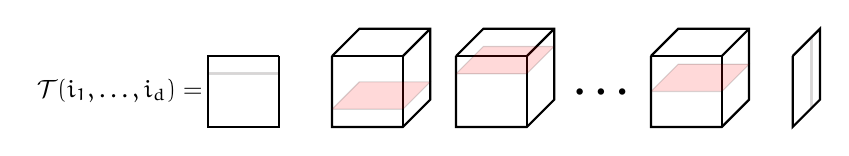
\begin{tikzpicture}[scale=.9]
			\draw[thick](0,2,1)--(0,2,0)--(1,2,0)--(1,1,0)--(1,1,1)--(0,1,1)--(0,2,1);
			\draw[thick](0,2,1)--(1,2,1)--(1,1,1);
			\draw[thick] (1,2,1)--(1,2,0);
			\draw[thick](1.75,2,1)--(1.75,2,0)--(2.75,2,0)--(2.75,1,0)--(2.75,1,1)--(1.75,1,1)--(1.75,2,1);
			\draw[thick](1.75,2,1)--(2.75,2,1)--(2.75,1,1);
			\draw[thick] (2.75,2,1)--(2.75,2,0);
			\node at (3.85,1.5, 1) {\begin{LARGE}$\dots$\end{LARGE}};		
			\draw[thick](4.5,2,1)--(4.5,2,0)--(5.5,2,0)--(5.5,1,0)--(5.5,1,1)--(4.5,1,1)--(4.5,2,1);
			\draw[thick](4.5,2,1)--(5.5,2,1)--(5.5,1,1);
			\draw[thick] (5.5,2,1)--(5.5,2,0);
			\draw[thick] (-.75,2,1)--(-1.75,2,1)--(-1.75,1,1)--(-.75,1,1)--(-.75,2,1);
			\draw[thick] (6.5,2,1)--(6.5,2,0)--(6.5,1,0)--(6.5,1,1)--(6.5,2,1);
			\node at (-3,1.5, 1) {\begin{small}$\mathcal T(i_1,\dots,i_d)=$\end{small}};
			
			\draw[very thick,fill=red,opacity=.15](-1.75,1.75,1)--(-0.75,1.75,1);
			\draw[fill=red,opacity=.15](0,1.25,1)--(1,1.25,1)--(1,1.25,0)--(0,1.25,0)--(0,1.25,1);
			\draw[fill=red,opacity=.15](1.75,1.75,1)--(2.75,1.75,1)--(2.75,1.75,0)--(1.75,1.75,0)--(1.75,1.75,1);
			\draw[fill=red,opacity=.15](4.5,1.5,1)--(5.5,1.5,1)--(5.5,1.5,0)--(4.5,1.5,0)--(4.5,1.5,1);
			\draw[very thick,fill=red,opacity=.15] (6.5,2,.3)--(6.5,1,.3);
		\end{tikzpicture}%
	\end{center}
	\end{onlyenv}%
	\begin{onlyenv}<2,4>
		\[
		\mathcal T(i_1,\dots,i_d)=\sum_{j_1=1}^{k_1}\dots\sum_{j_{d-1}=1}^{k_{d-1}}U_1(i_1, j_1)U_2(j_1,i_2,j_2)\dots U_d(j_{d-1}, i_d).
		\]
	\end{onlyenv}%
	\begin{onlyenv}<3>
	\[
	\mathcal T(i_1,\dots,i_d)=\vcenter{\hbox{
\includegraphics[width=0.65\columnwidth]{train.png}}}
	\]
\end{onlyenv}%
\begin{itemize}
	\item Smallest possible tuple $(k_1,\dots,k_{d-1})$ is called the \alert{\textbf{TT-rank}} of $\mathcal T$.
	\item $U_j\in\mathbb C^{k_{j-1}\times n_j\times k_j}$ are called the \alert{\textbf{TT cores}} of $\mathcal T$ (with $k_0=k_d=1$).
	\item If TT ranks are not large $\leadsto$ high compression ratio as $d$ grows.
	\item TT decomposition multilinear with respect to the cores.
\end{itemize}
\onslide<4>{If for any $1\leq \mu\leq d-1$ we group the first $\mu$ factors and last $d-\mu$ factors then
\[
\mathcal T({\color{blue}i_1,\dots,i_{\mu}},{\color{red}i_{\mu+1},\dots,i_d}),
\]
is the matrix-matrix product of two (large) matrices.
}

\end{frame}

\begin{frame}{\faTrain\;TT decomposition and matrix factorizations}
	The \alert{\textbf{$\mu$th unfolding}} of $\mathcal T\in\mathcal C^{n_1\times \dots\times n_d}$ is obtained by arranging the
	entries in a matrix
	$$
	T^{<\mu>}\in \mathbb C^{(n_1\cdots n_\mu)\times (n_{\mu+1}\cdots n_d)}
	$$
	where the corresponding index map is given by
	\begin{align*}
		\mathrm{ind}:\mathbb N^{n_1\times \dots\times n_d}\quad &\rightarrow\quad \mathbb N^{(n_1\cdots n_\mu)\times (n_{\mu+1}\cdots n_d)}\\
		\mathrm{ind}(i_1,\dots,i_d)\quad &=\quad  (i_{row},i_{col}),
	\end{align*}
	where
	\begin{align*}
		i_{row}&=1 + \sum_{s=1}^{\mu}(i_s-1)\prod_{t=1}^{s-1}n_t,\\
		i_{col}&=1 + \sum_{s=\mu+1}^{d}(i_s-1)\prod_{t=\mu+1}^{s-1}n_t
	\end{align*}
\end{frame}

\begin{frame}{\faTrain\;TT decomposition and matrix factorizations}
We can compute the \textbf{compression} of the \textbf{tensor} by computing the SVD of the \emph{unfoldings}.
\begin{alertblock}{Lemma \parencite{MR2837533}}
	The \alert{\textbf{TT rank}} of a tensor $\mathcal T$ is given by\vspace{-1em}
	\[
	\operatorname{tt-rank}(\mathcal T)=(\operatorname{rank}(T^{<1>}),\dots,\operatorname{rank}(T^{<d-1>})).
	\]
\end{alertblock}
\begin{columns}
\begin{column}{0.75\columnwidth}\small
\begin{algorithm}[H]
\KwIn{Tensor $\mathcal T$, ranks $k_1,\dots,k_d)$}
\KwOut{$U_1,\dots,U_d$.}
$k_0=k_d=1$\;
\For{$\mu=1,\dots,d-1$}{
Reshape $\mathcal T$ into $T^{<2>}\in\mathbb C^{k_{\mu-1}n_\mu\times (n_{\mu+1}\dots n_d)}$\;
Compute rank-$k_\mu$ approximation $T^{<2>}\approx U\Sigma V^T$ (e.g. via SVD)\;
Reshape $U$ into $U_{\mu}\in\mathbb C^{k_{\mu-1}\times n_\mu\times k_\mu}$\;
Update $\mathcal T$ via $T^{<2>}\gets U^T X^{<2>}=\Sigma V^T$\;
}
Set $U_d=\mathcal T$\;
\caption{\textsc{TT-SVD}$(\mathcal T, k_1,\dots,k_d)$}
\end{algorithm}
\end{column}
\begin{column}{0.24\columnwidth}
\faBook\;The \alert{\textbf{proof}} is obtained by simply following the steps of the algorithm.

\faHammer\;We can use \emph{tolerances} instead of fixed ranks.
\end{column}
\end{columns}
\end{frame}

\begin{frame}{\faTrain\;TT decomposition and matrix factorizations}
And we can estimate the resulting error using the best approximation properties of the SVD.
\begin{alertblock}{Theorem \parencite{MR2837533}}
Let $\mathcal T_{SVD}$ denote the tensor in TT decomposition obtained from
TT-SVD. Then
\[
\|{\mathcal T-\mathcal T_{SVD}}\|\leq \sqrt{\epsilon_1^2+\dots +\epsilon_d^2}
\]
where
\[
\epsilon_\mu^2 =\|{T^{<\mu>}- U\Sigma V^T}\|_F^2=\sigma_{k_\mu+1}^2+\sigma_{k_\mu+2}^2+\dots\ .
\]
\end{alertblock}

\begin{itemize}
	\item[\faCog] We can modify the algorithm to accommodate different compression algorithms than the SVD,
	\item[\faCog] We can also compute the approximation via sketching algorithms, and avoiding using all the entries of $\mathcal{T}$.
\end{itemize}

\end{frame}

\begin{frame}{\faTrain\;TT-Matrices and matrix-vector products}
If a \textbf{vector of length} $N = n_1\times\ldots\times n_d$ is treated as a \textbf{$d$--dimensional tensor}
with mode sizes $n_k$, and represented in TT--format, the \alert{\textbf{matrices
acting on it}} have the form
\begin{equation*}
	\mathcal{M}(\alert<2>{i_1,\ldots,i_d},\alert<3>{j_1,\ldots,j_d}) = M_1(i_1,j_1)\ldots M(i_d,j_d), \qquad M_k(i_k,j_k) \in \mathbb{R}^{r_{k-1}\times r_k},\vspace{-1em}
\end{equation*}
\begin{itemize}
	\item[\faCogs]<2-> the first block indexes $i_1,\ldots,i_d$ enumerate the rows,
	\item[\faCogs]<3-> the second block indexes $j_1,\ldots,j_d$ enumerate the columns.
\end{itemize}

\onslide<3->{Given $\mathcal{M}$ in TT--format, and a vector $\mathcal{X}$ in
$TT$--format with cores $X_k$, and entries $X(j_1,\ldots,j_d)$ then
the \alert{\textbf{matrix--vector multiplication}} amounts to the following sum
\begin{equation*}
	\mathcal{Y}(i_1,\ldots,i_d) = \sum_{j_1,\ldots,j_d} \mathcal{M}(i_1,\ldots,i_d,j_1,\ldots,j_d) \mathcal{X}(j_1,\ldots,j_d) = Y_1(i_1)\ldots Y_{d}(i_d),
\end{equation*}
where $Y_k(i_k) = \sum_{j_k} M_k(i_k,j_k) \otimes X_k(j_k)$ \onslide<4->{\alert<4>{\faExclamationTriangle}\,The ranks of $\mathcal{Y}$ are the product of the
	ranks of the matrix and of the vector! So we need to \textbf{recompress} after every matrix-vector product.}}

\end{frame}

\begin{frame}[fragile]{\faTrain\;TT-representation for our case}

\begin{columns}
\begin{column}{0.5\columnwidth}
\begin{itemize}
	\item[\faCog] We can use the same routine as before to \emph{represent} the two BVM matrices,
	\item[\faCog]<2-> We build a tensor in which all the modes have size $2$, this is usually called a Quantized-TT (QTT) formulation:
\begin{onlyenv}<2->
\definecolor{bg}{rgb}{0.95,0.95,0.95}
\begin{minted}[bgcolor=bg,fontsize=\small,breaklines]{matlab}
tA=tt_matrix(full(A),1e-14);
tA=tt_reshape(tA,2*ones(kval,2));
\end{minted} 
\end{onlyenv}
	\item[\faHammer]<3-> If we look at the values of $k$ and maximal $\operatorname{tt-rank}$ we find:\\[1em]
	
	\begin{tabular}{l|lllllll}
	k & 2 & 3 & 4 & 5 & 6 & 7 & 8 \\\midrule
	$\max(\operatorname{tt-rank}(\mathcal{A}))$ & 3 & 5 & 6 & 7 & 7 & 7 & 9 \\
	\end{tabular}
\end{itemize}
\end{column}
\begin{column}{0.5\columnwidth}
\definecolor{bg}{rgb}{0.95,0.95,0.95}
\begin{minted}[bgcolor=bg,fontsize=\small,breaklines]{matlab}
%% Time-dependent operator
kval = 5;       % Grid power
m = 2^kval;     % Number of time steps
k = 2;
[Alpha,Beta] = mab(k,m);
A = Alpha(:,2:m+1);
B = Beta(:,2:m+1);
t0 = 0;
tf = 1;
h = (tf-t0)/m;
tA = tt_matrix(full(A),1e-14);
tA = tt_reshape(tA,2*ones(kval,2));
tB = tt_eye(2,kval);
\end{minted}
\end{column}
\end{columns}

\end{frame}

\begin{frame}[fragile]{\faTrain\;TT-representation for our case}
\begin{columns}
	\begin{column}{0.5\columnwidth}
\begin{itemize}
	\item[\faHammer] We can act similarly also for the space operator.
	\item[\alert{\faExclamationTriangle}]<2-> We could be way more clever in the representation of these matrices, these are diagonal times Toeplitz, and we could do something specialized, \emph{e.g.}, \parencite{MR3066807}.
\end{itemize}
	\end{column}
	\begin{column}{0.5\columnwidth}
\definecolor{bg}{rgb}{0.95,0.95,0.95}
\begin{minted}[bgcolor=bg,fontsize=\small,breaklines]{matlab}
%% Compression of the space part
tL = tt_matrix(L,1e-14);
tL = tt_reshape(tL,2*ones(kval+1,2));
tM = tt_eye(2,kval+1);
%% Final assembly
tMat = tkron(tA,tM)-h*tkron(tB,tL);
\end{minted}
	\end{column}
\end{columns}

\begin{itemize}
	\item[\faQuestionCircle]<3-> Now that we have everything in this format, how can we solve our problem?
\end{itemize}
\begin{description}
	\item[TT-GMRES]<4-> An option is to rephrase our favorite Krylov method using the TT arithmetic, \parencite{MR3043559} and adapt what we know to build a preconditioner~\parencite{MR3936774}.
	\item[AMEn]<5-> Use a \emph{specialized solver} for linear systems in TT format~\parencite{MR3262607}.
\end{description}

\end{frame}

\begin{frame}[fragile]{\faCross\;Concluding with an AMEn}

Using AMEn~\parencite{MR3262607} as \definecolor{bg}{rgb}{0.95,0.95,0.95}\vspace{-0.5em}
\begin{minted}[bgcolor=bg,fontsize=\small,breaklines]{matlab}
tx = amen_solve2(tMat,ttb,1e-6);
\end{minted}

\begin{onlyenv}<2>
\begin{center}
\begin{tabular}{rrrrrl}
\toprule
k & $m$ & $n$ & IT & Residual & $\max(\operatorname{tt-rank}(\mathcal{A}))$ \\
\midrule
2 & 64 & 128 & 9 & 2.231e-07 & 22 \\
2 & 128 & 256 & 10 & 3.428e-07 & 26\\
2 & 256 & 512 & 14 & 5.925e-07 & 30 \\
2 & 512 & 1024 & 22 & 3.957e-07 & 33 \\
2 & 1024 & 2048 & 35 & 6.034e-07 & 37 \\
2 & 2048 & 4096 & 47 & 6.968e-07 & 42 \\ 
\bottomrule
\end{tabular}
\end{center}
\end{onlyenv}
\begin{onlyenv}<3->
	\begin{center}
		\begin{tabular}{rrrrrl}
			\toprule
		k & $m$ & $n$ & IT & Residual & $\max(\operatorname{tt-rank}(\mathcal{A}))$ \\
		\midrule
3 & 64 & 128 & 8 & 2.252e-07 & 20 \\
3 & 128 & 256 &  11 & 2.153e-07 & 24 \\
3 & 256 & 512 & 15 & 2.138e-07 & 28 \\
3 & 512 & 1024 & 18 & 2.950e-07 & 32 \\
3 & 1024 & 2048 & 35 & 8.961e-07 & 36 \\
3 & 2048 & 4096 & 50 & 3.821e-06 & 44 \\
\bottomrule
\end{tabular}
\end{center}
\end{onlyenv}

\begin{itemize}
	\item[\faEye]<4-> Behavior is \emph{similar} to the matrix-equation solver,
	\item[\faHammer]<5-> We could play around with different \textbf{settings} and \textbf{options} of the AMEn solver.
	\item[\faBinoculars]<6-> Studying the right combination of parameters, representation, setups is still an open problem for the BVM all-at-once approaches.
\end{itemize}

\end{frame}

\section{Conclusion and summary}

\begin{frame}{Conclusion and summary}
	\definecolor{success}{HTML}{4a934a}
	\definecolor{todo}{HTML}{0099cc}
	
	\begin{itemize}
		\item[\textcolor{success}{\faCheckCircle}] We have seen how to work with linear multistep methods in boundary value form,
		\item[\textcolor{success}{\faCheckCircle}] We have discussed some structured preconditioning strategy for the resulting linear systems,
		\item[\textcolor{success}{\faCheckCircle}] We have introduced the machinery for working with tensor equations in the Tensor Train format.
		\item[\faBinoculars] There are \emph{many} open problems and possibilities to do better here.
	\end{itemize}
	\vfill
	
	Next up
	\begin{itemize}
		\item[\textcolor{todo}{\faClipboardList}] Fractional Laplacians,
		\item[\textcolor{todo}{\faClipboardList}] Rational approximations and matrix functions,
		\item[\textcolor{todo}{\faClipboardList}] A couple of applications to complex network theory.
	\end{itemize}
	
\end{frame}

	{\unnumbered
		\begin{frame}[allowframebreaks,noframenumbering]{Bibliography}
			\small
			\printbibliography
			
		\end{frame}
	}
\end{document}